\chapter{初段ミューオントリガーの性能評価}\label{chapter5}
\ref{L1Topo}節で述べたL1 Triggerには、ミューオンの不変質量を指針としたトリガーを持つL1Topoが存在する。しかし、不変質量を計算するときに使用するミューオンの運動量は、L1Muonから送られてくる$p_{\rm{T}}$閾値であるため、L1Muonの$p_{\rm{T}}$閾値の細かさがそのままL1Topoのトリガー性能に影響する。
そこで、Run-3ではL1Muonにおける判定可能な$p_{\rm{T}}$閾値を6段階から15段階に増設することで、より細かい精度での$p_{\rm{T}}$判定を可能とし、L1 Trigger全体としてのトリガー性能の向上を図った。
したがって、本研究で作成するCWにも正確に15段階の$p_{\rm{T}}$判定ができることが要求される。

本章では、第~\ref{chapter4}章で述べた手法を用いて作成した2種類のCW(シミュレーション用のCWと実際の測定用のCW)を用いたトリガーの性能の評価を行う。

\section{機械学習を用いて作成したCWの15段階閾値の評価}
便宜上、本研究の手法で作成した2種類のCWについて、シミュレーション用のCWを$\mathrm{CW_{Simu}}$、実際の測定用のCWを$\mathrm{CW_{Data}}$と呼び、比較対象として2022年度Run-3で使用されたCWを$\mathrm{CW_{2022}}$と呼ぶこととする。

まず、全オフライン再構成されたミューオンの内、ある$p_{\rm{T}}$閾値以上のトリガーが発行された割合$\epsilon$を計算し、トリガー効率の算出を行った。また、$\epsilon$をオフライン再構成した$p_{\rm{T}}$の関数として表したTurn-on curveを描き、式~\eqref{equ:fitting}の関数によってフィッティングを行う事で、トリガー性能の評価を行った。
このとき、Tag$\&$Probe法を用いて評価に用いるデータの処理を行う。
\subsubsection{Tag$\&$Probe法}
実際の実験データはトリガーによって選別された粒子の情報のみが保存されているため、そのままのデータを用いてトリガーの性能評価を行うとバイアスがかかる可能性がある。そこで、このバイアスを除く手法としてTag$\&$Probe法を用いる。

Tag$\&$Probe法では、一般的に$Z$ボゾンや$J/\psi$粒子の崩壊で生じた2つのミューオンを使用し評価を行う。崩壊由来の2つのミューオンのうち、片方のミューオン(Tag)が事象選択のトリガーとしてトリガーが発行された場合、もう一方のミューオン(Probe)をトリガー効率の評価に用いる。Probeミューオンに対してトリガーが発行されたかを見ることで、実際の測定でトリガーによって取得されたミューオンというバイアスをなくしてトリガー効率を見積もることができる。

本研究では、内部飛跡検出器とミューオン検出器でそれぞれ独立にオフライン再構成されたZボソン由来のミューオンを用いて評価を行う。1回の衝突事象に対し、2つ以上のミューオン候補が存在するイベントのみを用いる。それらのミューオン候補のうち、任意の2つの電荷が異符号となっているミューオンペアを選び出し、不変質量を再構成する。再構成した不変質量が80 GeV$<M_Z<$100~GeVであることを要求することでZボソン由来のミューオンと判断する。
これらのミューオンのうち、一方をTagミューオン、もう一方をProbeミューオンと定義する。
まず、Tagミューオンがトリガーを発行したかどうかを判定する。Run-2での実験データを解析に使用する際のトリガー判定には、HLTのシングルミューオントリガーである「HLT$\_$mu26$\_$ivarmeduium」を使用する。
ここでトリガー発行の判定を行うために $\Delta R= \sqrt{(\Delta \eta)2 + (\Delta \phi)2}$を定義する。
ここで$\Delta\eta$, $\Delta\phi$はデータに保存されているトリガーを発行した飛跡情報と、オフライン再構成されたTagミューオンの$\eta$方向、$\phi$方向の差分である。
図~\ref{fig:tag_HLT}にTag ミューオンとHLTの$\Delta R$を$p_{\rm{T}}$の関数として表した2次元分布を示す。
本研究では$\Delta R< 0.001$を満たせばTagミューオンがトリガーを発行したとみなす。
TagミューオンがHLTを発行しているとみなされた時、もう一つのミューオンをProbeミューオンとして使用する。Probeミューオンはデータ保存のために発行されたトリガーとは独立なミューオンであるためバイアスの影響はない。

\begin{figure}[htb]
  \centering
  %\rule{8cm}{6cm}
  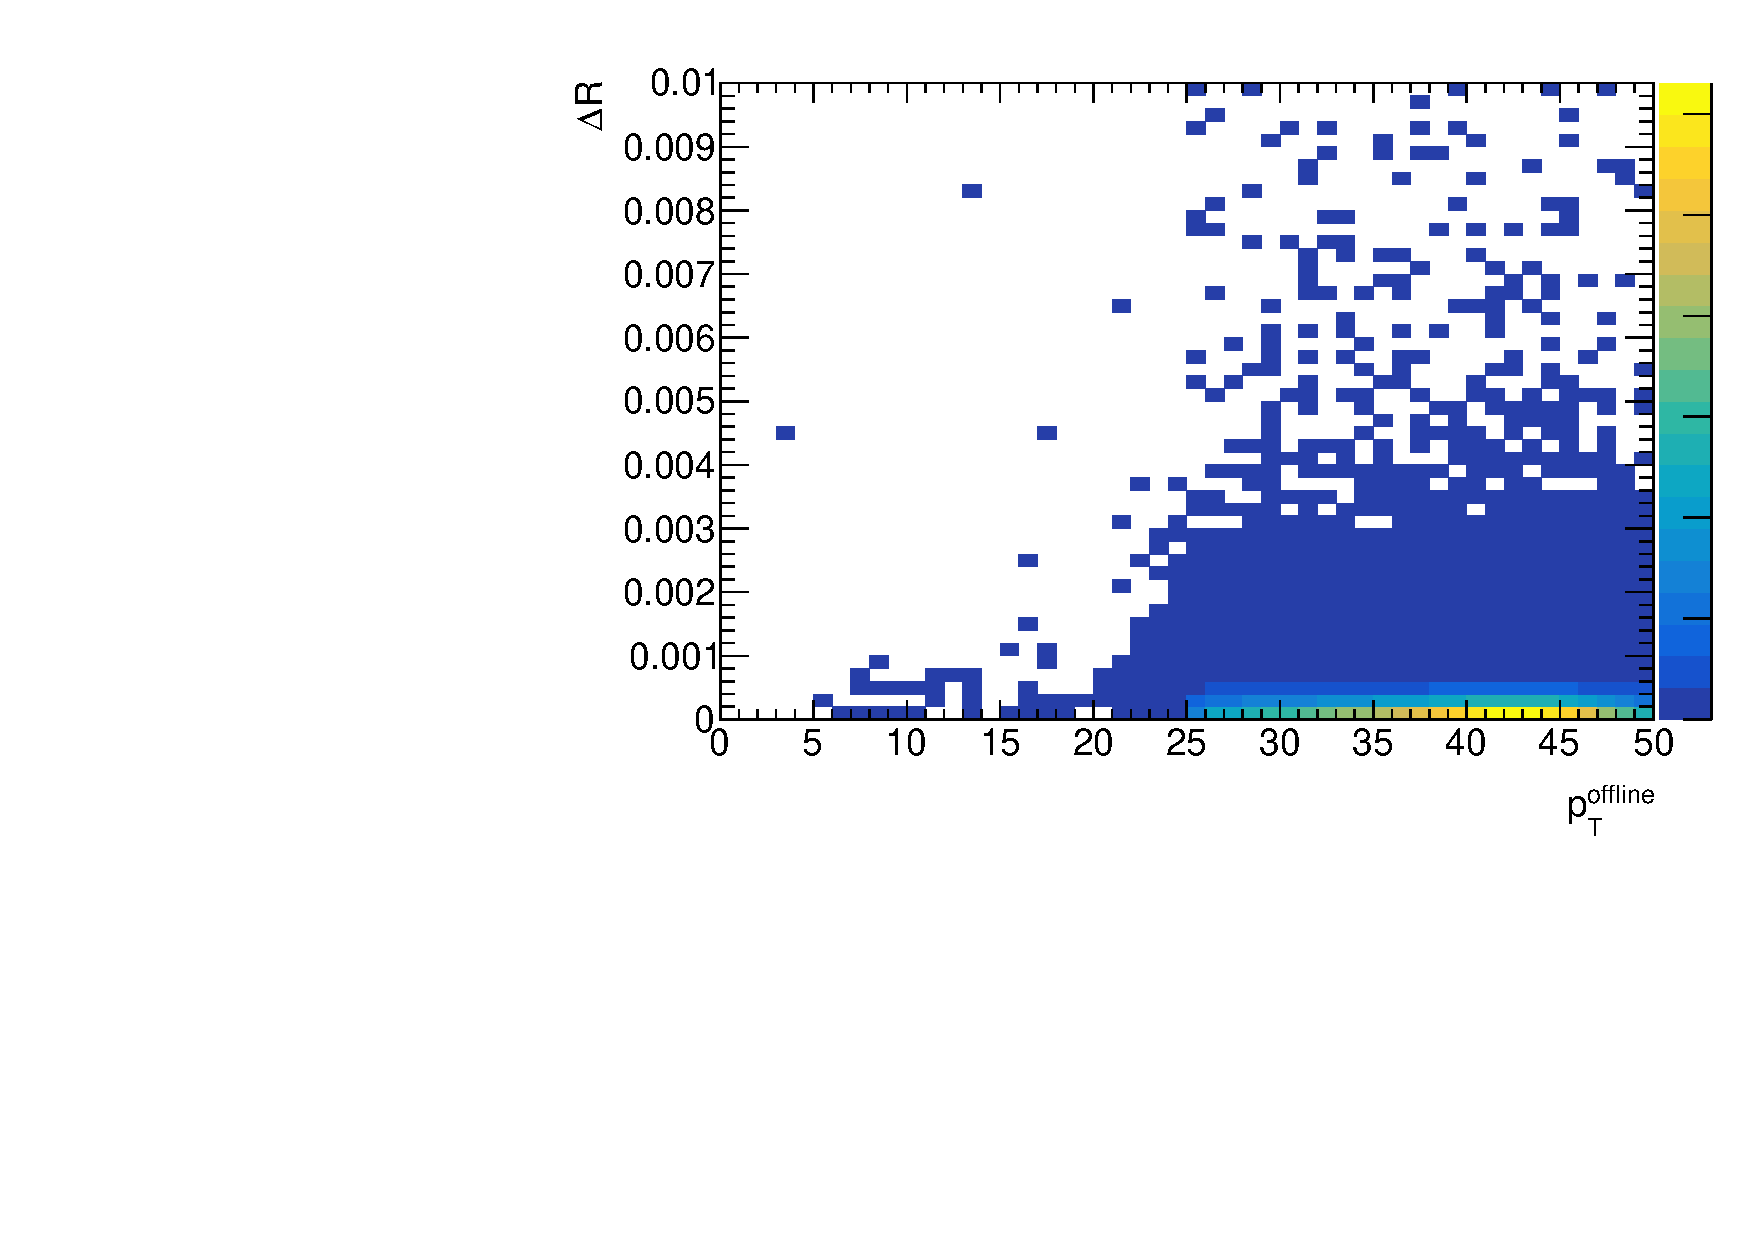
\includegraphics[clip, width=11cm]{fig/3/dR_tag_HLT.pdf}
  \caption{TagミューオンとHLTの$\Delta R$分布。$\Delta R<0.001$ならばTagミューオンがHLTを発行したものとする。}
  \label{fig:tag_HLT}
\end{figure}

次に、Probeミューオンを使用してエンドキャプ部のトリガー性能を評価するために、Probe ミューオンとTGCのヒット情報を一致させる。図~\ref{fig:Probe_TGC}にProbeミューオンとTGCのヒット情報の$\Delta R$を$p_{\rm{T}}$の関数として表した2次元分布を示す。本研究では$\Delta R<0.04$を満たせばProbeミューオンがTGCのヒット情報と一致したものとする。
このProbeミューオンの情報と一致したTGC のヒット情報を使って評価を行う。

\begin{figure}[htb]
  \centering
  %\rule{8cm}{6cm}
  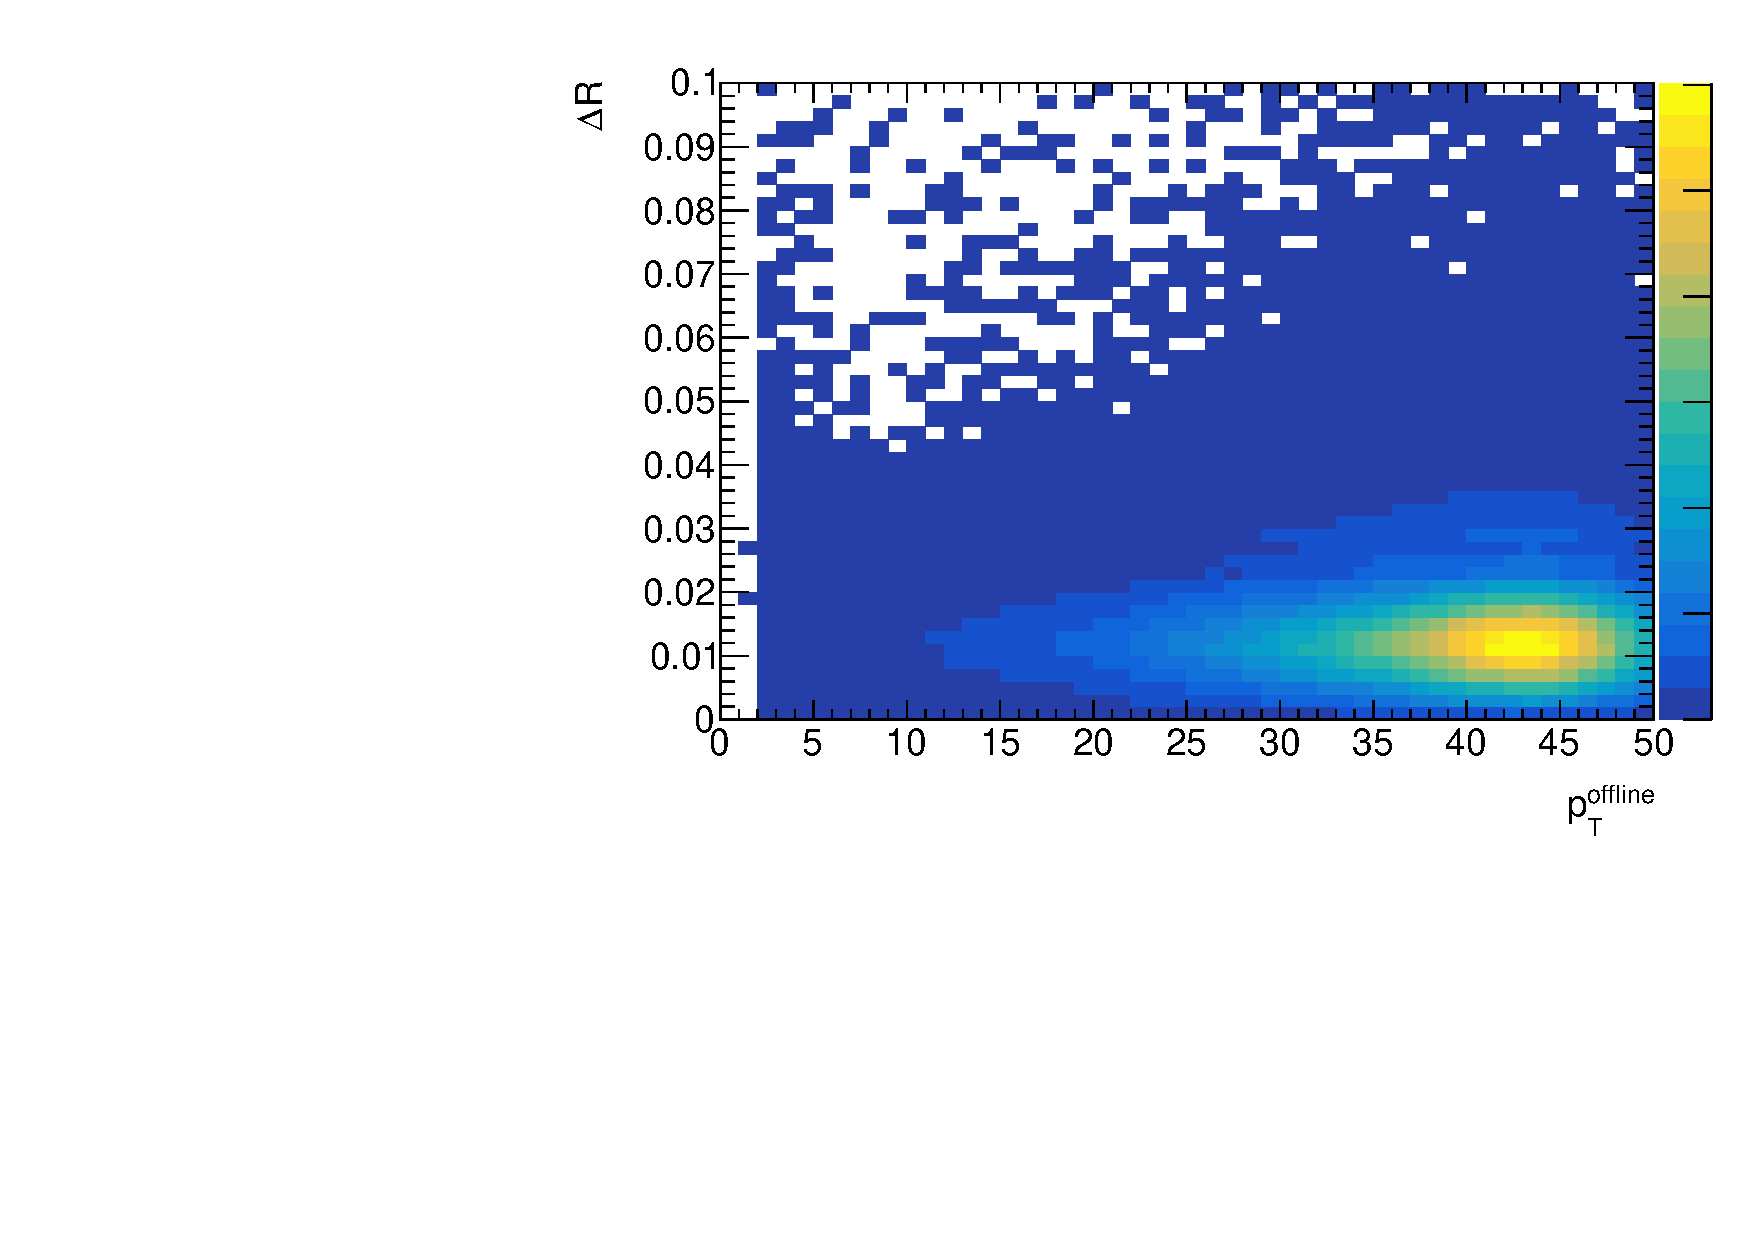
\includegraphics[clip, width=11cm]{fig/3/dR_probe_RoI.pdf}
  \caption{ProbeミューオンとTGCのヒット情報との$\Delta R$分布。$\Delta R< 0.04$ならばProbeミューオンがTGCのヒット情報と一致したものとする。}
  \label{fig:Probe_TGC}
\end{figure}

\subsection{作成したCWの15段階の$p_{\rm{T}}$閾値}
図~\ref{fig:15Eff_CW_Data}に$\mathrm{CW_{Data}}$を用いて15段階の$p_{\rm{T}}$閾値におけるTurn-on curveを示す。評価には2018年Run-2 のデータに対して$Z\rightarrow \mu\mu$によるTag$\&$Probe法を用いた。
$\mathrm{CW_{2022}}$と同様に、本研究の手法で作成した$\mathrm{CW_{Data}}$は15段階に分かれたTurn-on curveを描けていることがわかる。
また、図~\ref{fig:15Eff_CW_Simu}に$\mathrm{CW_{Simu}}$を用いてを要求した15段階の$p_{\rm{T}}$閾値におけるTurn-on curveを示す。評価にはシングルミューオンのシミュレーションサンプルを用いた。
比較のため、図~\ref{fig:Run3_15_MC5} に $\mathrm{CW_{2022}}$を用いた15段階の$p_{\rm{T}}$閾値におけるのTurn-on curveを示す。
こちらも同様に、本研究の手法で作成した$\mathrm{CW_{Simu}}$は15段階に分かれたTurn-on curveを描けていることがわかる。
よって、本研究の手法によって作成された2種類のCWは、2022年度Run-3において使用された$\mathrm{CW_{2022}}$と同様に15段階の判定が可能であることが見て取れる。
\begin{figure}
    %\centering
    \begin{tabular}{cc}
    \begin{minipage}[b]{0.45\hsize}
        %\centering
        \hspace*{-1cm}
        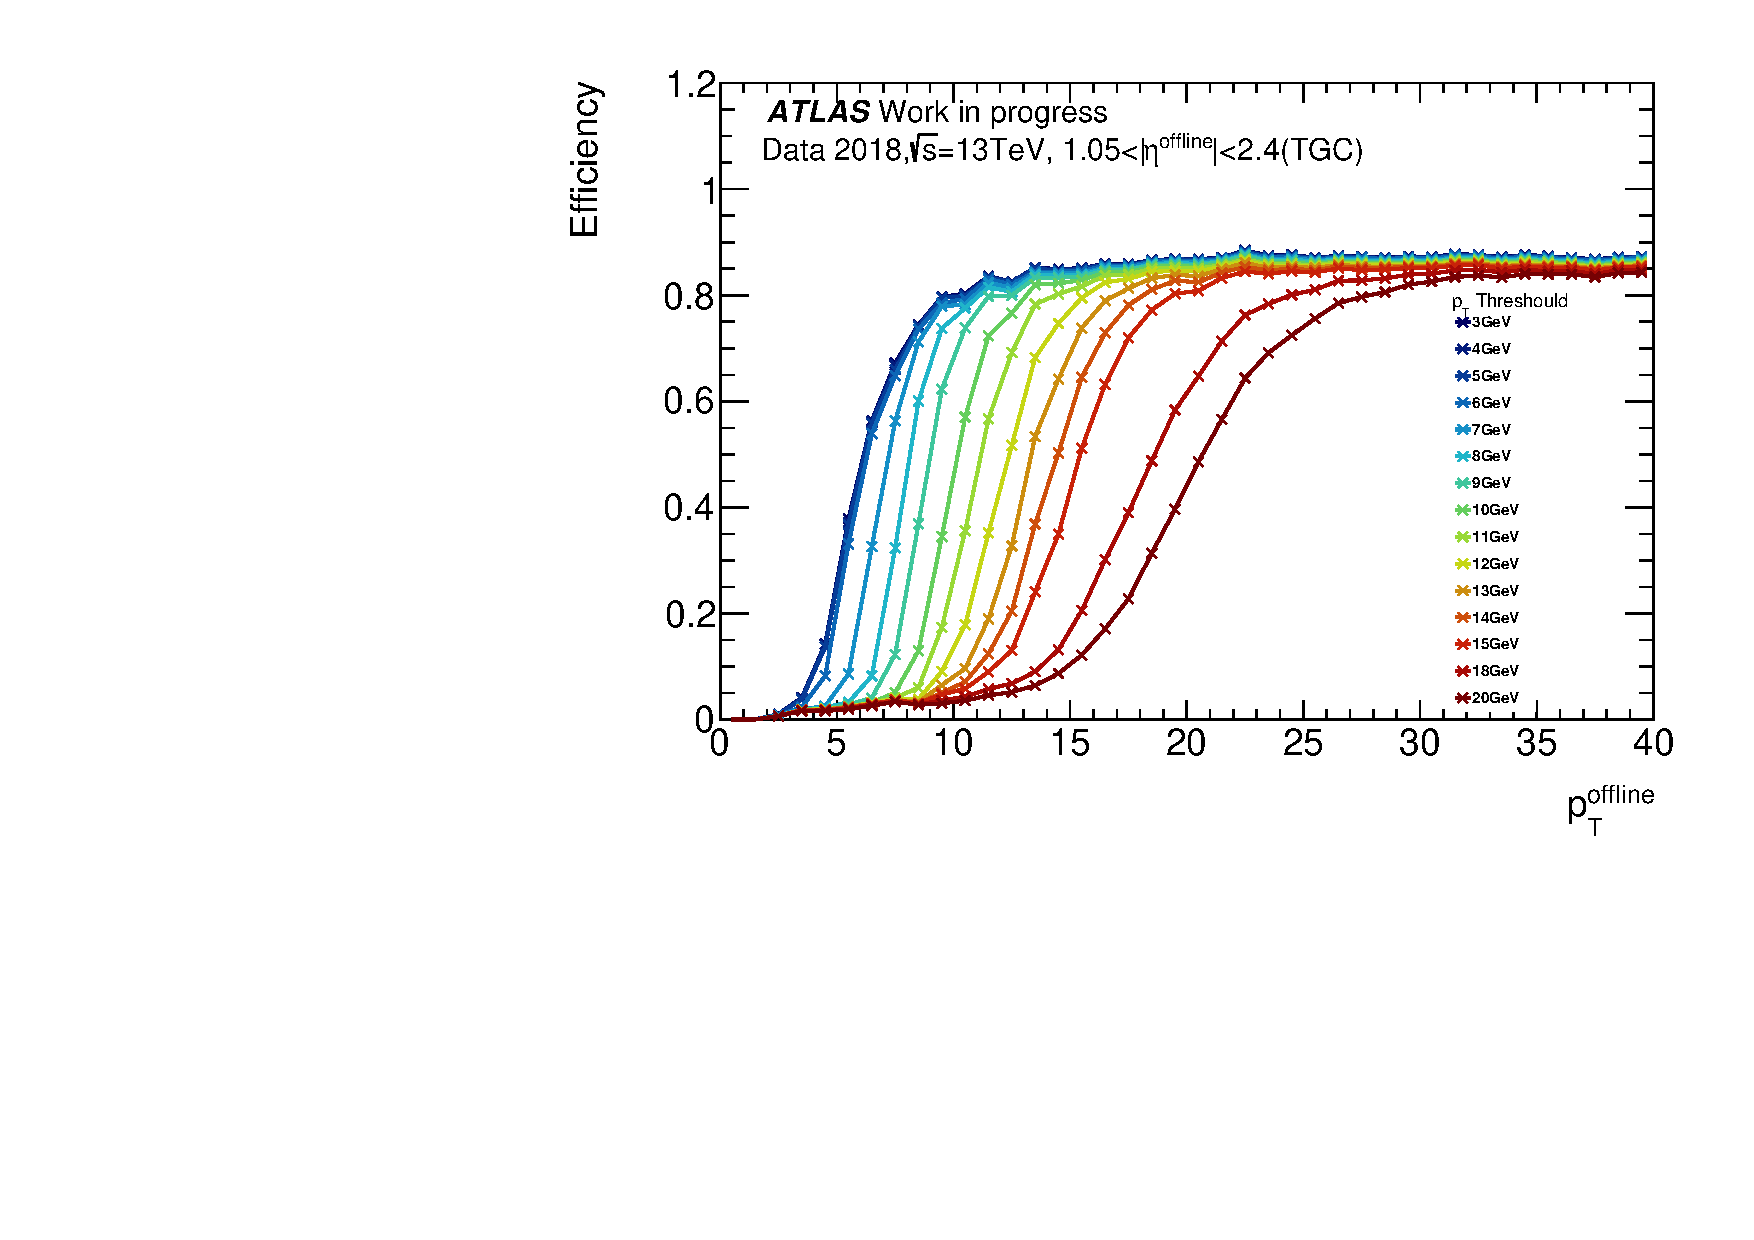
\includegraphics[clip, width=8cm]{fig/5/15_v06_Data.pdf}
        %\vspace{5pt}
        \subcaption{}
        \label{fig:15Eff_CW_Data}
    \end{minipage}&
    %\hfill
    \begin{minipage}[b]{0.45\hsize}
        %\centering
        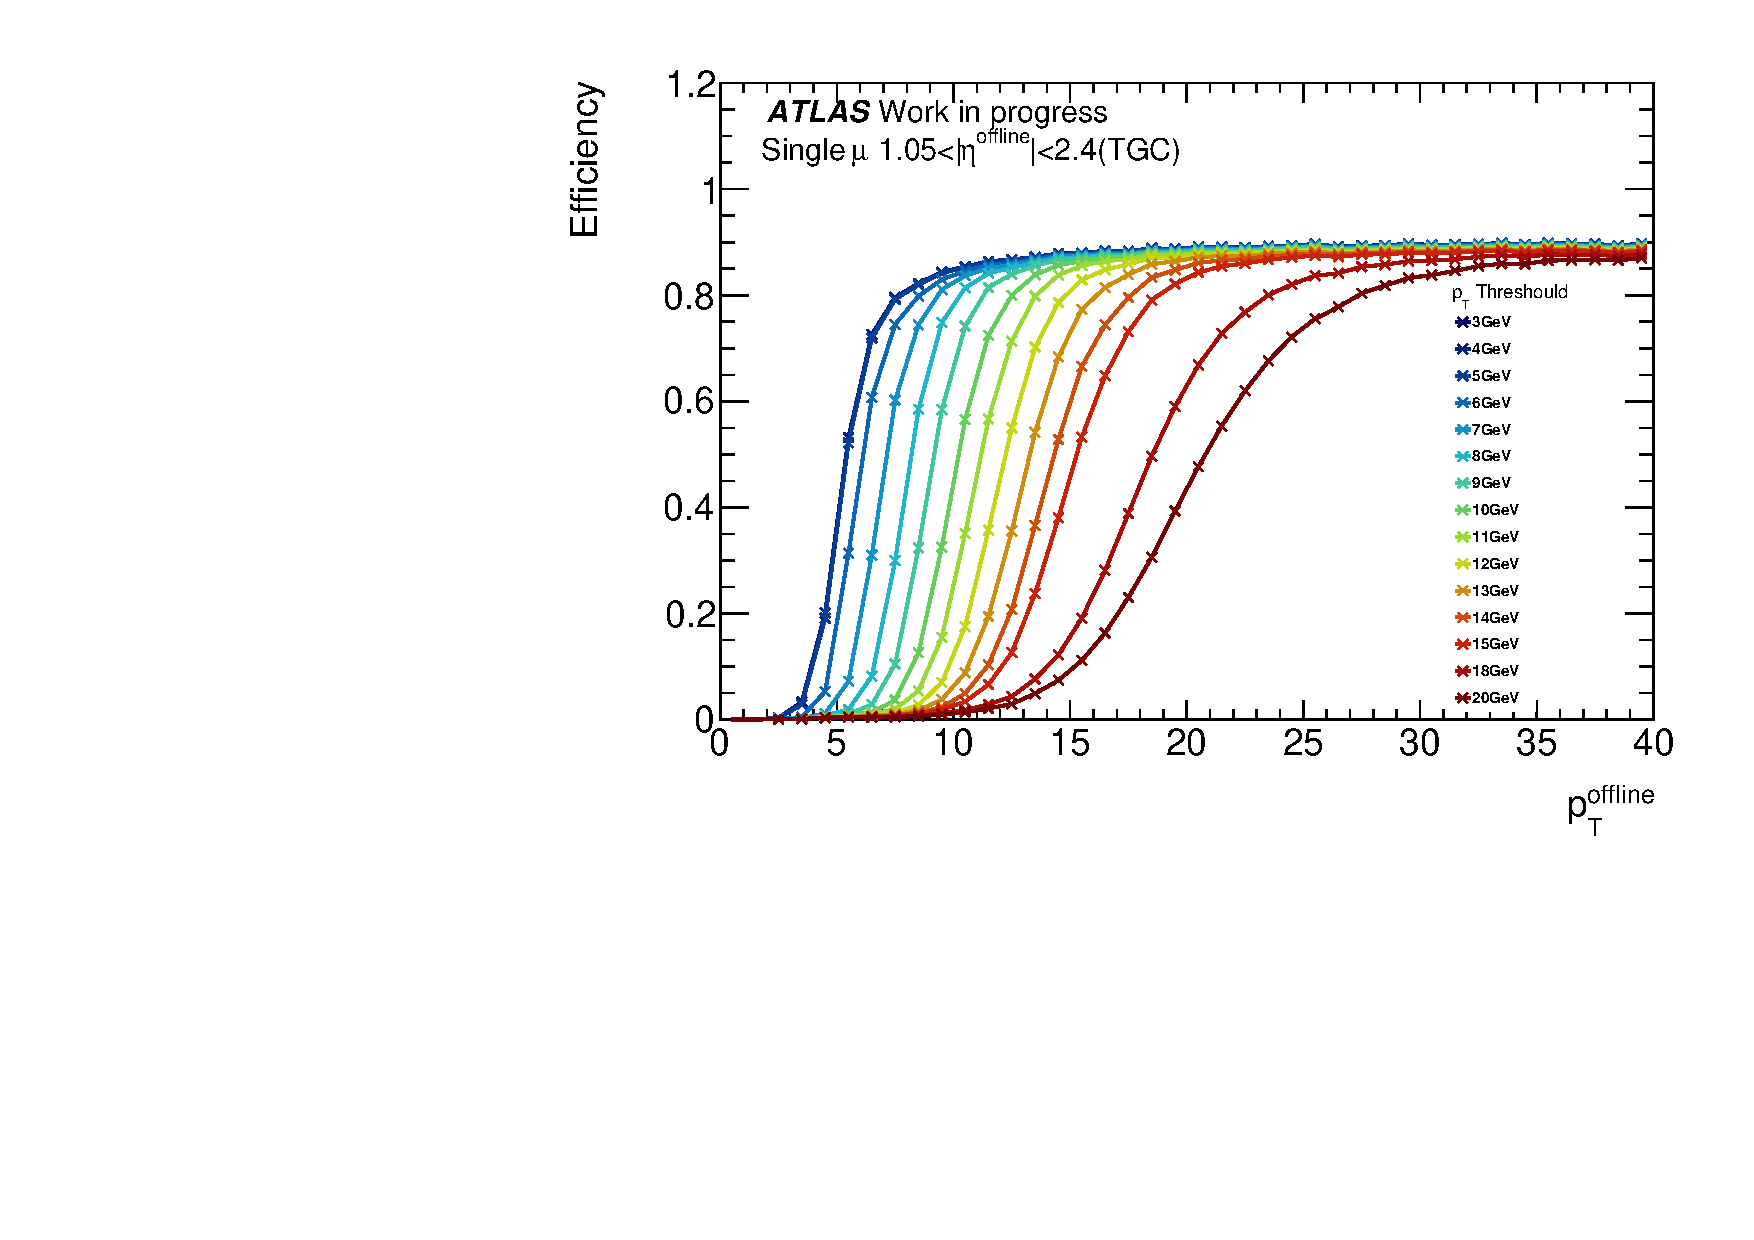
\includegraphics[clip, width=8cm]{fig/5/15_MC_MC.pdf}
        %\vspace{5pt}
        \subcaption{}
        \label{fig:15Eff_CW_Simu}
    \end{minipage}
    \end{tabular}
    \caption{機械学習を用いて作成したCWの15段階の閾値におけるTurn-on curve。(a):実際のデータを用いてトレーニングを行った機械学習から作成したCW。(b): シミュレーションデータを用いてトレーニングを行った機械学習から作成したCW。}
    \label{}
\end{figure}

\begin{figure}[tb]
  \centering
  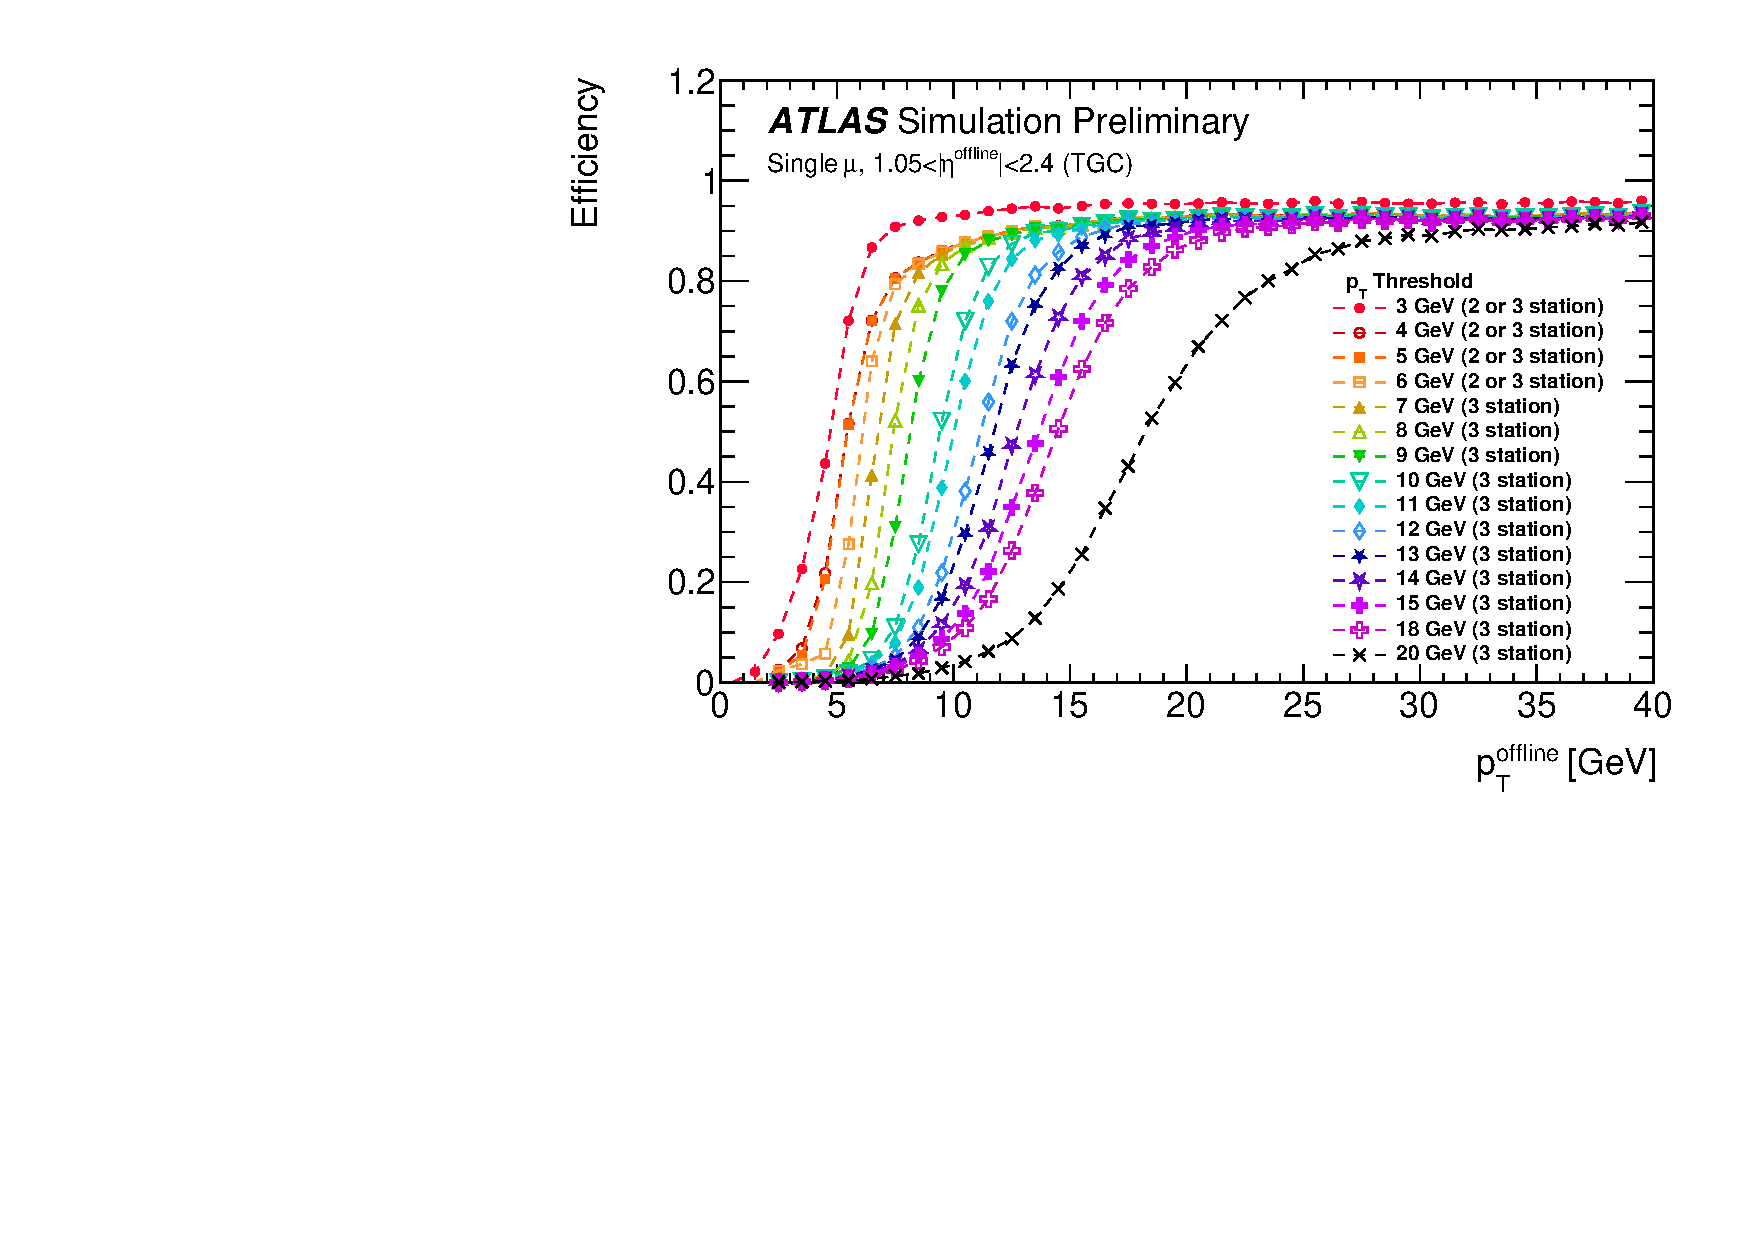
\includegraphics[clip, width=10cm]{fig/3/PLOT-TRIG-2020-01-fig1.pdf}
  \caption{2022年Run-3で使用した15段階閾値のTurn-on curve。シングルミューオンのシミュレーションサンプルに対してのトリガー効率を示している。}
  \label{fig:Run3_15_MC5}
\end{figure}

\subsection{現行のトリガーとのトリガー性能の比較}
次に、それぞれの15段階の$p_{\rm{T}}$閾値のトリガーについて評価を行う。

\subsubsection{トリガー効率の評価}
まず、$\mathrm{CW_{Simu}}$と$\mathrm{CW_{2022}}$のトリガー効率$\epsilon$を比較する。評価にはシングルミューオンのシミュレーションデータを用いる。

図~\ref{fig:v05v07} には$p_{\rm{T}}$閾値が14~GeVの時の、$\mathrm{CW_{2022}}$と$\mathrm{CW_{Simu}}$のTurn-on curveの比較を示す。
2022年度Run-3で使用されている$\mathrm{CW_{2022}}$に比べて、本研究の手法ので作成した$\mathrm{CW_{Simu}}$の方がTurn-on curveの立ち上がりが鋭くなっており、トリガー性能が良くなっていることが見て取れる。
また、他の$p_{\rm{T}}$閾値における比較を図~\ref{fig:v05v07_1_9_Simu}及び図~\ref{fig:v05v07_12_20_Simu}に示す。
15段階の閾値において、本研究の手法によって作成された$\mathrm{CW_{Simu}}$は、2022年度Run-3において使用された$\mathrm{CW_{2022}}$と同様に鋭く立ち上がっていることが見て取れる。
\begin{figure}[htb]
  \centering
  %\rule{8cm}{6cm}
  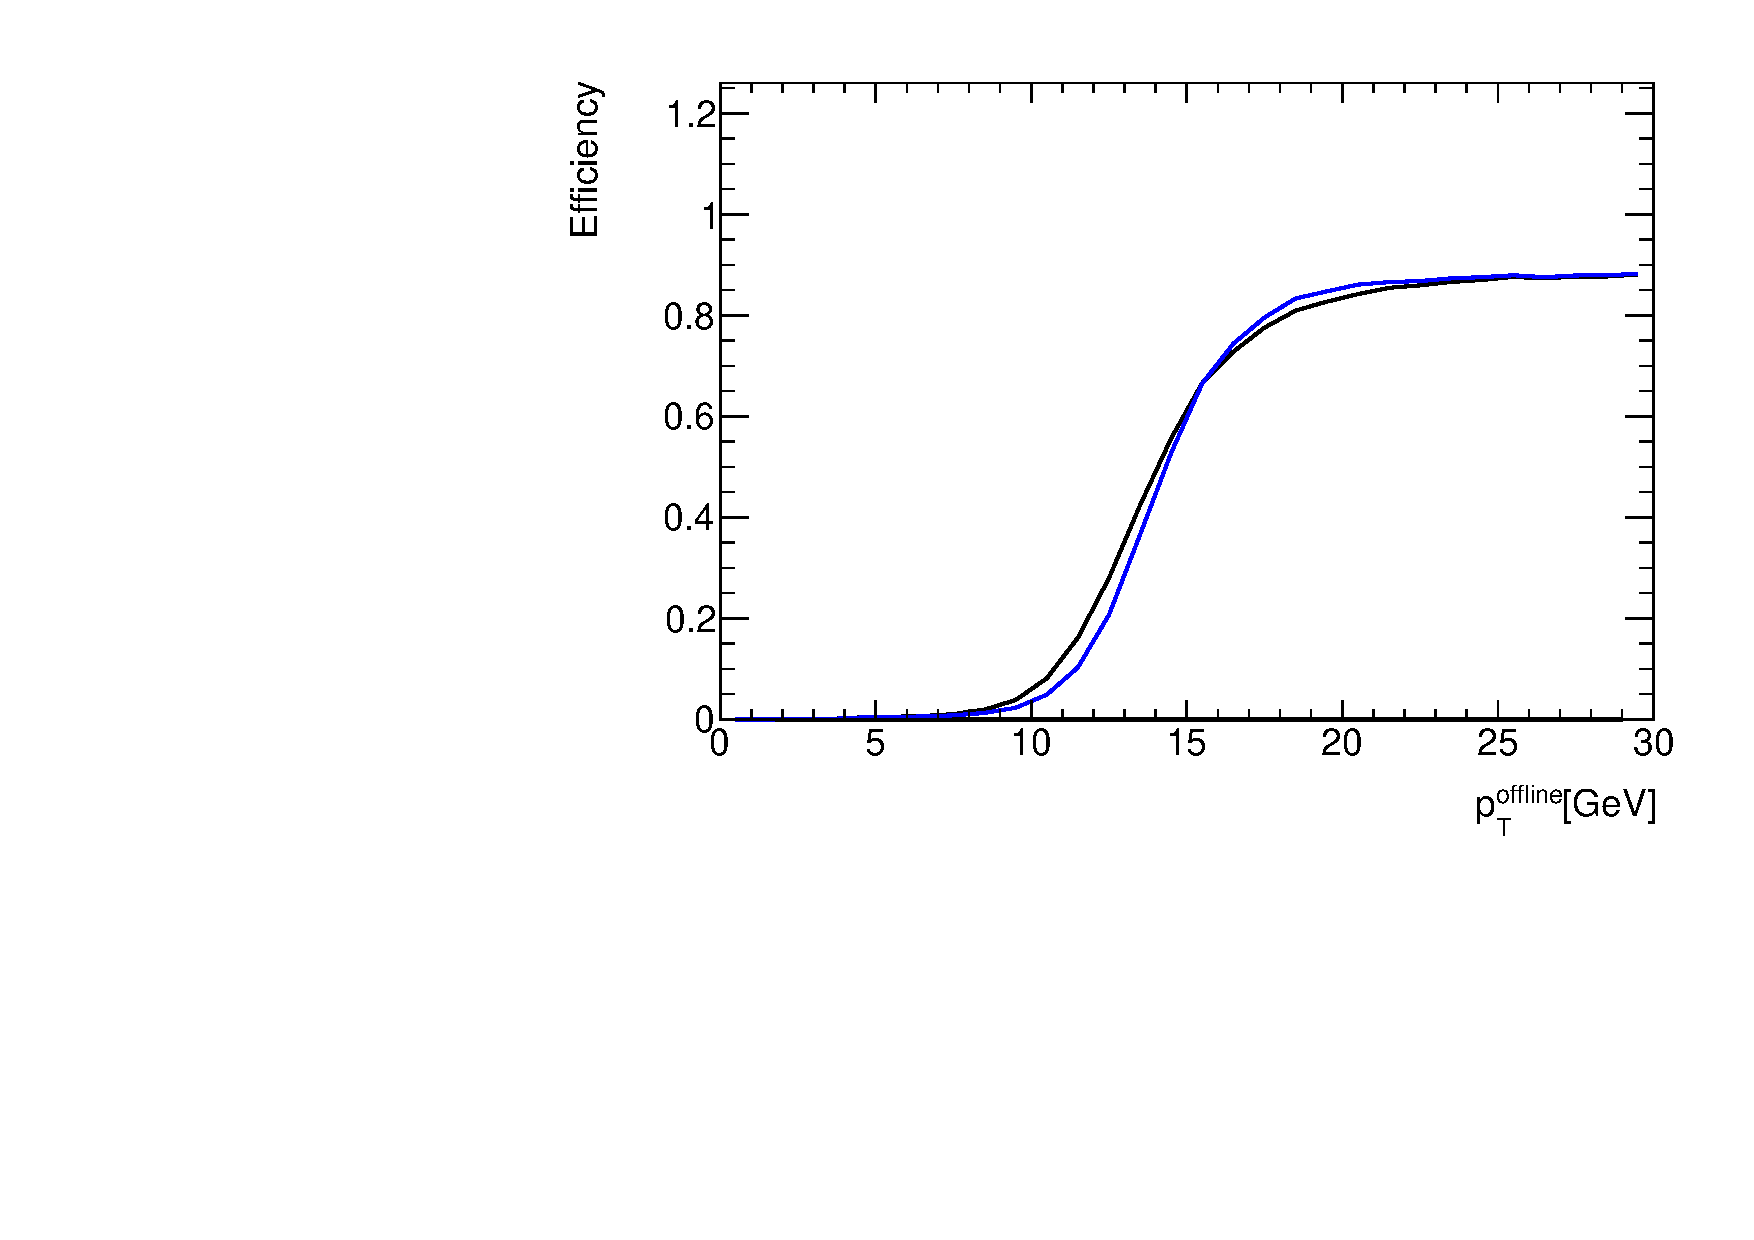
\includegraphics[clip, width=10cm]{fig/5/v05vsv07_MU14.pdf}
  \caption{$p_{\rm{T}}$閾値14~GeVにおける$\mathrm{CW_{Simu}}$と$\mathrm{CW_{2022}}$のTurn-on curveの比較。評価にはシングルミューオンのシミュレーションデータを使用した。}
  \label{fig:v05v07}
\end{figure}

\begin{figure}[htb]
  \centering
  %\rule{8cm}{6cm}
  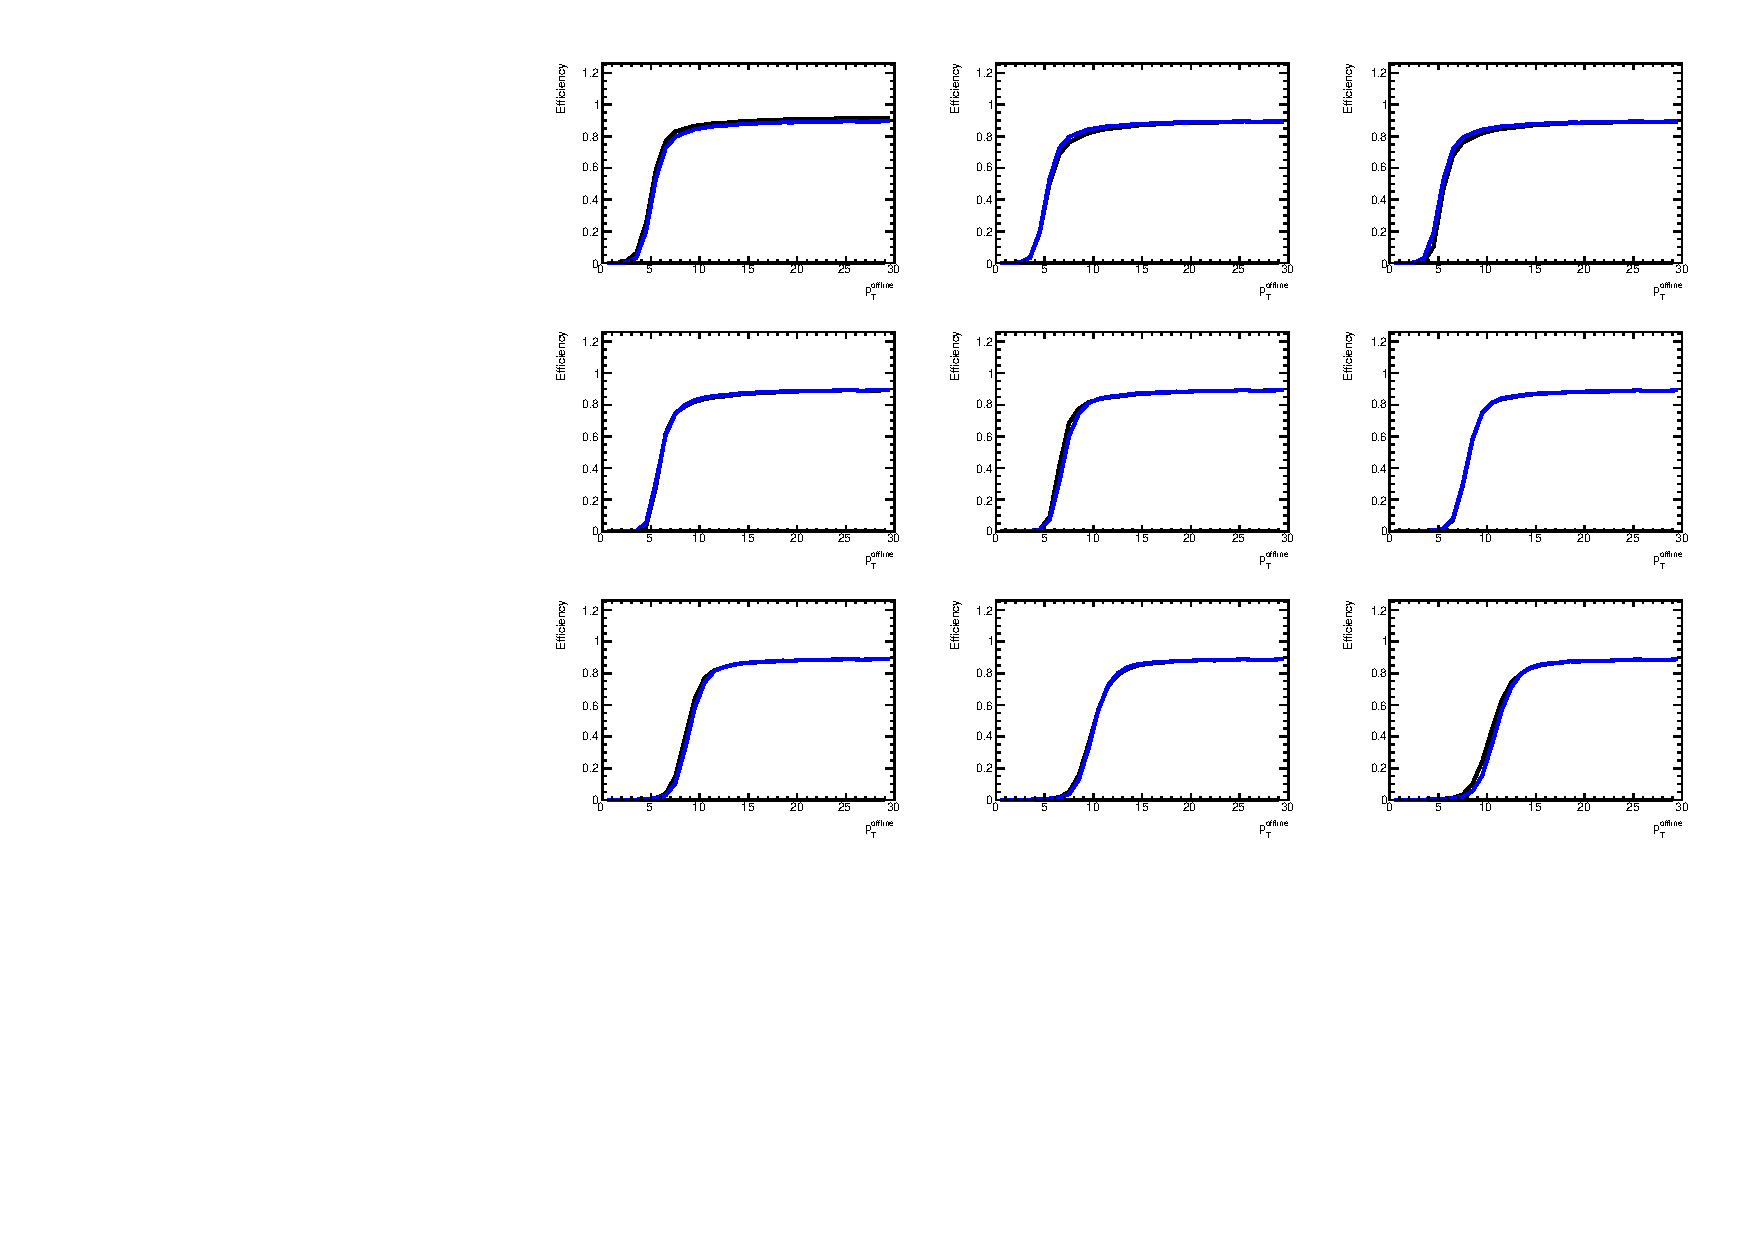
\includegraphics[clip, width=10cm]{fig/5/v05v07_1_9.pdf}
  \caption{$p_{\rm{T}}$閾値3~GeV$\sim$9~GeVにおける$\mathrm{CW_{Simu}}$と$\mathrm{CW_{2022}}$のTurn-on curveの比較。評価にはシングルミューオンのシミュレーションデータを使用した。}
  \label{fig:v05v07_1_9_Simu}
\end{figure}

\begin{figure}[htb]
  \centering
  %\rule{8cm}{6cm}
  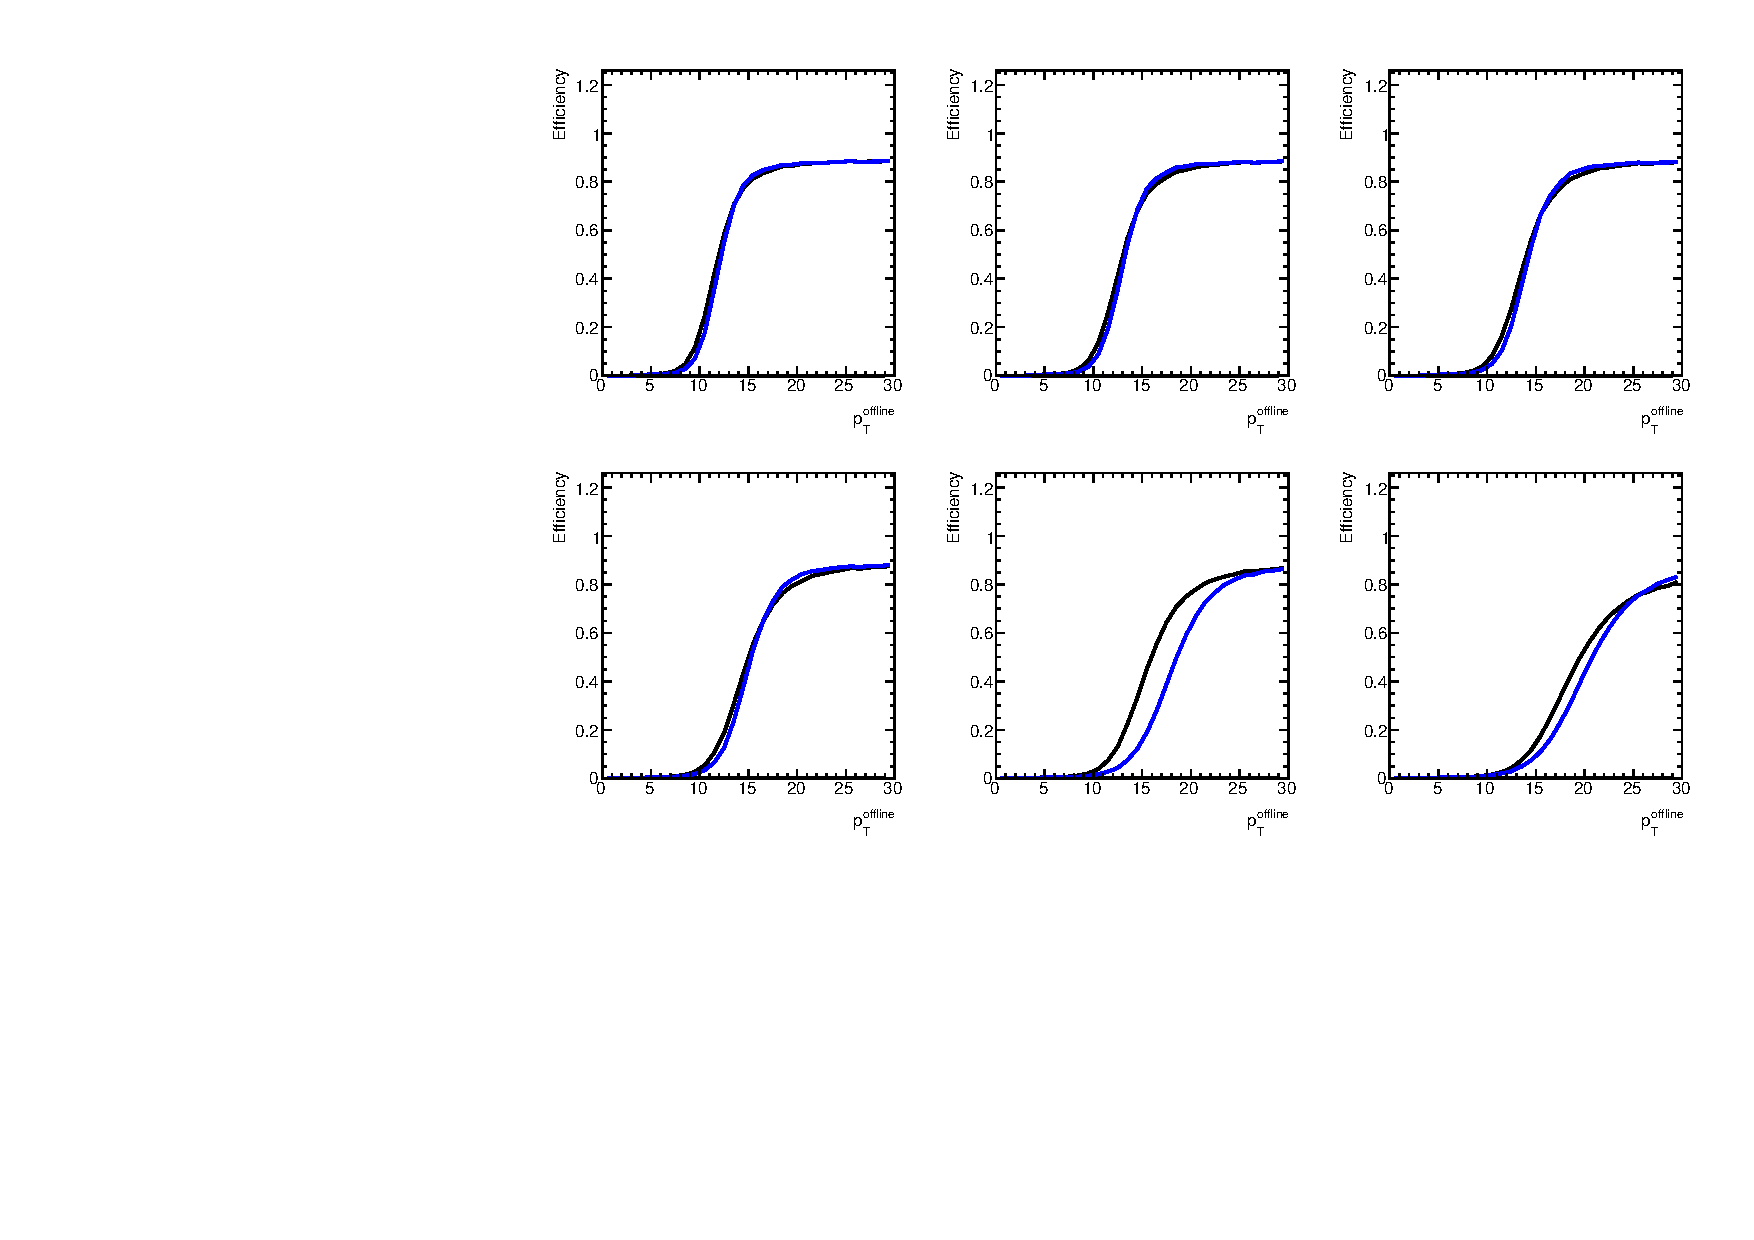
\includegraphics[clip, width=10cm]{fig/5/v05v07_10_15.pdf}
  \caption{$p_{\rm{T}}$閾値10~GeV$\sim$20~GeVにおける$\mathrm{CW_{Simu}}$と$\mathrm{CW_{2022}}$のTurn-on curveの比較。評価にはシングルミューオンのシミュレーションデータを使用した。}
  \label{fig:v05v07_12_20_Simu}
\end{figure}

さらに、これらのTurn-on curveに式~\eqref{equ:fitting}によるフィッティングを行い、パラメータの比較を行う。

図~\ref{fig:Resolution_v07v05}に$\mathrm{CW_{Simu}}$と$\mathrm{CW_{2022}}$のEffective thresholdに対するResolitionの比較を示す。
$\mathrm{CW_{Data}}$は全体的にResolutionの値が小さくなっており、Resolutionの改善がみられる。しかし、低いEffective thresholdのトリガーにおいては悪化が見られた。
これは***

図~\ref{Plateau_v07v05}に$\mathrm{CW_{Simu}}$と$\mathrm{CW_{2022}}$のEffective thresholdに対するPlateau Efficiencyの比較を示す。2018年Run-3で使用された$\mathrm{CW_{2022}}$と比べて、本研究の手法で作成した$\mathrm{CW_{Simu}}$は全体的にPlateau Efficiencyが向上している。
\begin{figure}[htb]
  \centering
  %\rule{8cm}{6cm}
  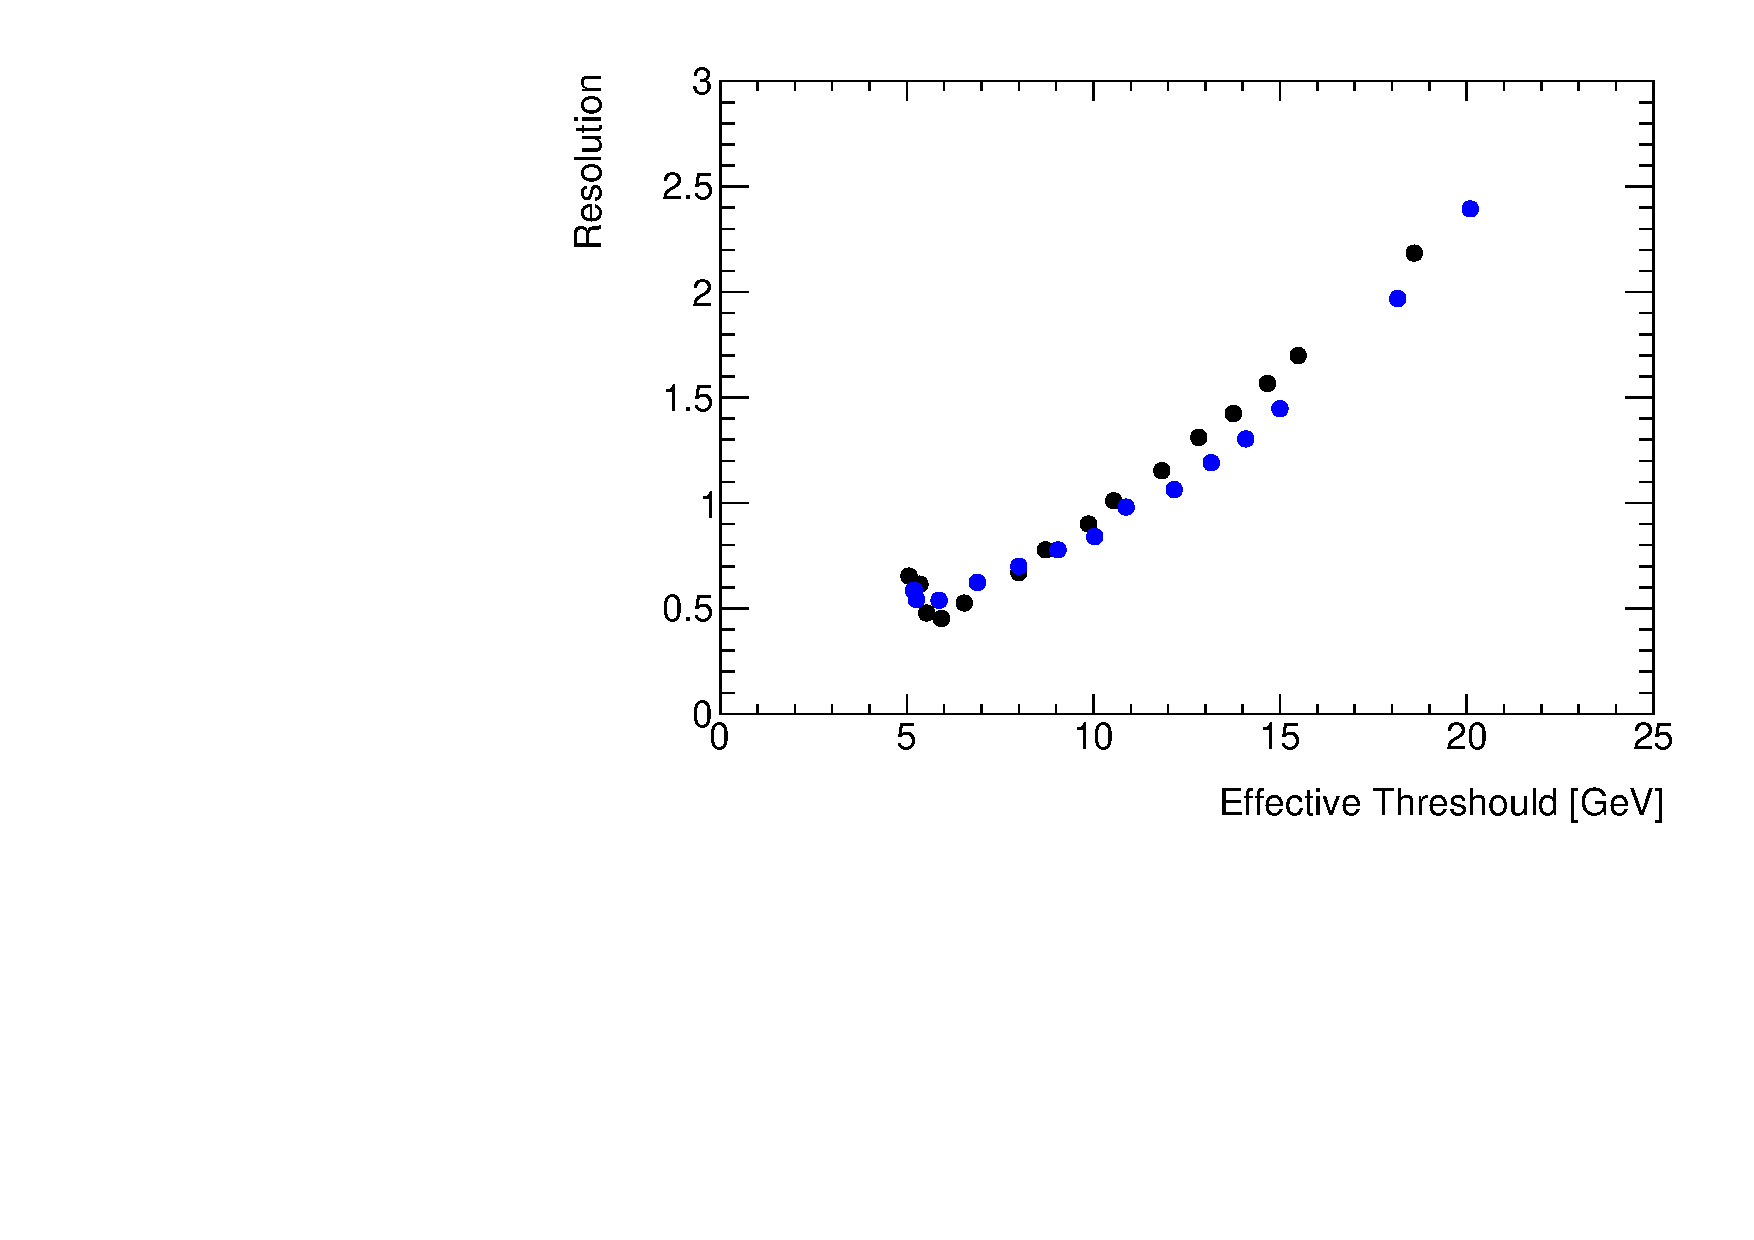
\includegraphics[clip, width=10cm]{fig/4/v05vsv07_Resolution.pdf}
  \caption{各Effective thresholdにおけるResolutionの比較。}
  \label{fig:Resolution_v07v05}
\end{figure}

\begin{figure}[htb]
  \centering
  %\rule{8cm}{6cm}
  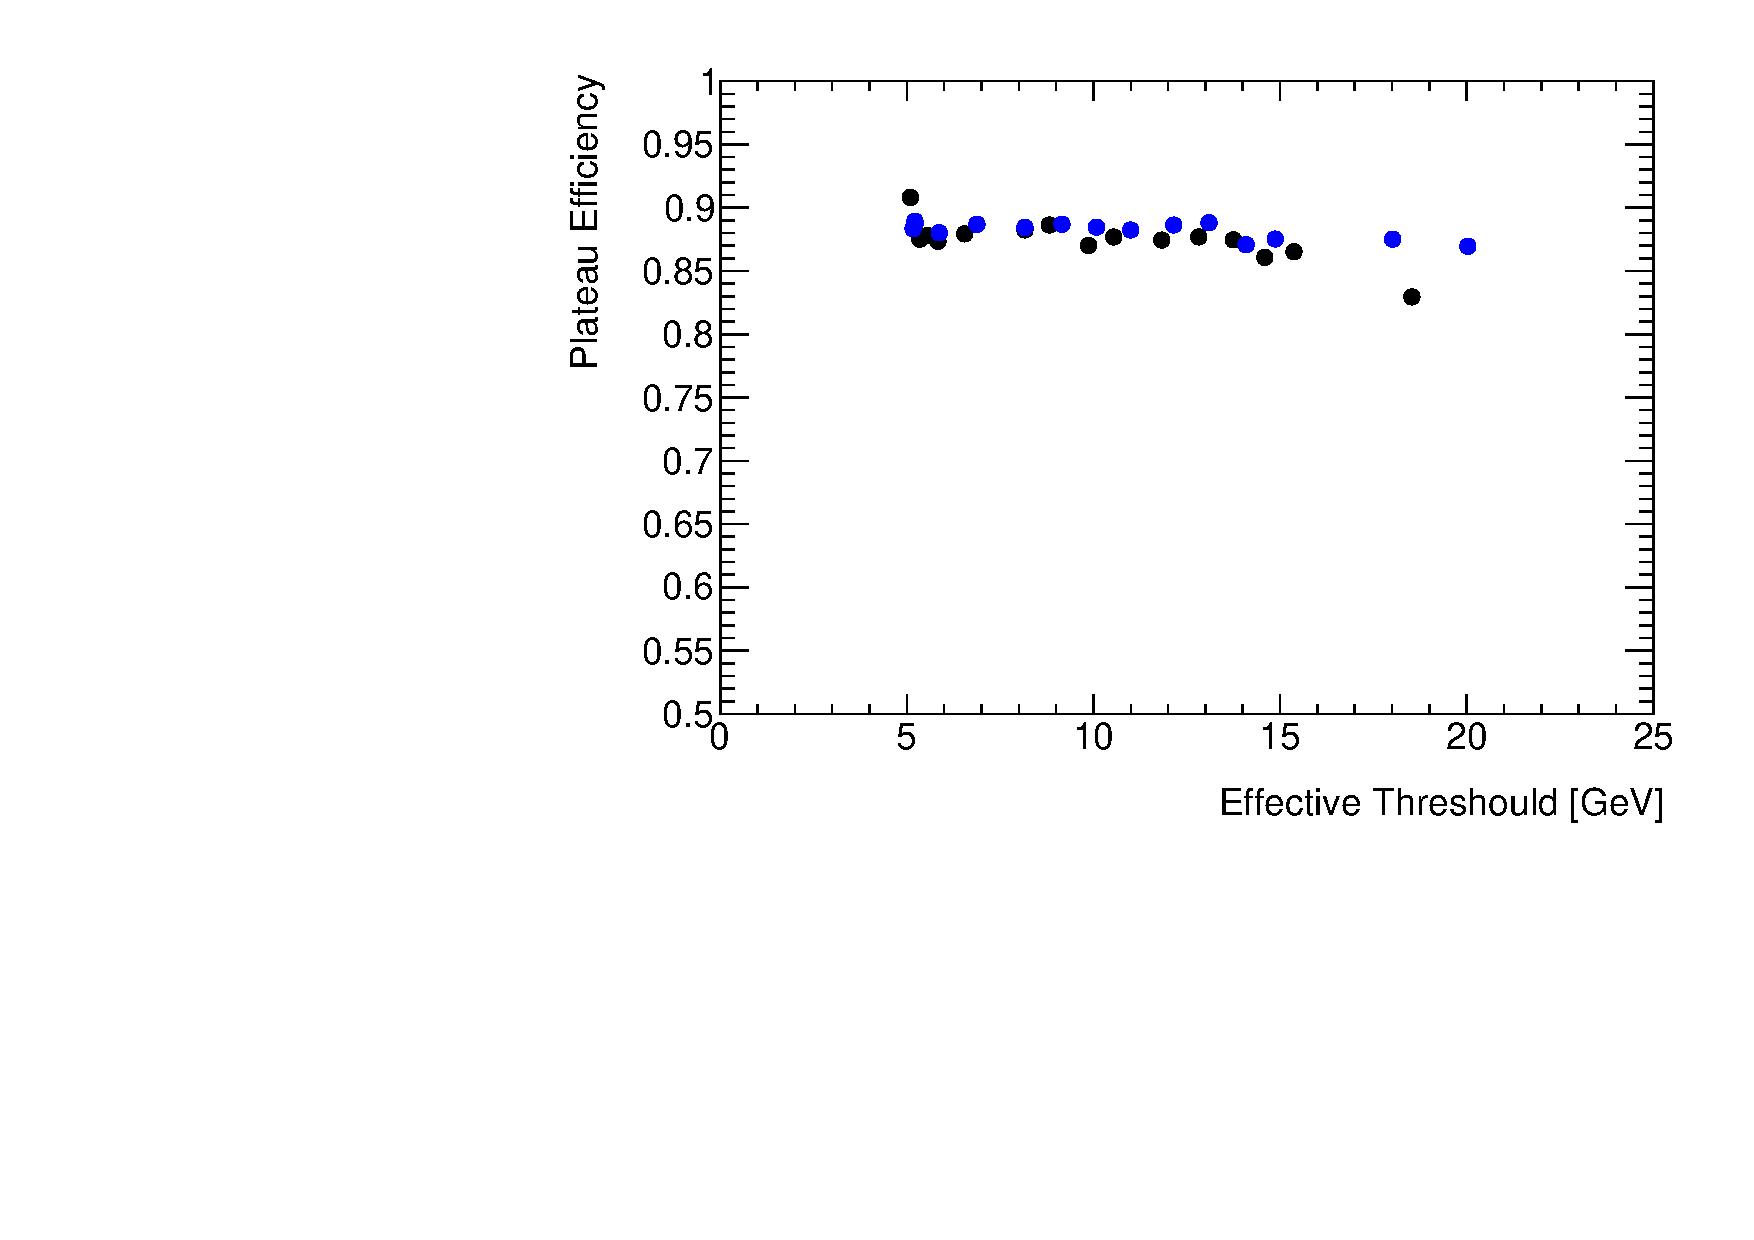
\includegraphics[clip, width=10cm]{fig/4/v05vsv07_Plateau.pdf}
  \caption{各Effective thresholdにおけるPlateau Efficiencyの比較。}
  \label{Plateau_v07v05}
\end{figure}

\subsubsection{$p_{\rm{T}}^{offline}$分解能の評価}
$p_{\rm{T}}$分解能を式~\eqref{equ:residual}で計算する$p_{\rm{T}}$ residualを用いて評価する。
\begin{equation}
    p_{\rm{T}} residual = \frac{p_{\rm{T}}^{L1}-p_{\rm{T}}^{offline}}{p_{\rm{T}}^{offline}}
    \label{equ:residual}
\end{equation}
ここで、$p_{\rm{T}}^{L1}$はL1MuonでCWを用いて判定される$p_{\rm{T}}$閾値、$p_{\rm{T}}^{offline}$はオフライン再構成されたミューオンで$p_{\rm{T}}$ある。
そのため、$p_{\rm{T}}^{offline}$に対して正しく$p_{\rm{T}}^{L1}$を判定できていれば0に近づき、0から離れるほど$p_{\rm{T}}^{L1}$が$p_{\rm{T}}^{offline}$とずれていることになる。

この$p_{\rm{T}}$ residualを1~GeVごとの$p_{\rm{T}}^{offline}$に対して計算し、細かい$p_{\rm{T}}$に対する分解能を見る。
まず、本研究の手法で作成した$\mathrm{CW_{Simu}}$と2022年度Run-2で使用された$\mathrm{CW_{2022}}$の比較を行う。
評価にはシングルミューオンのシミュレーションサンプルを用いる。
図~\ref{residual_MC_3_10}と図~\ref{residual_MC_11_18}に1~GeVごとの$p_{\rm{T}}^{offline}$に対する$p_{\rm{T}}$ residual分布を示す。
本研究の手法で作成した$\mathrm{CW_{Simu}}$は、2022年度Run-3で使用された$\mathrm{CW_{2022}}$と同様の分布を示している。
\begin{figure}[htb]
  \centering
  %\rule{8cm}{6cm}
  \hspace*{-1cm}
  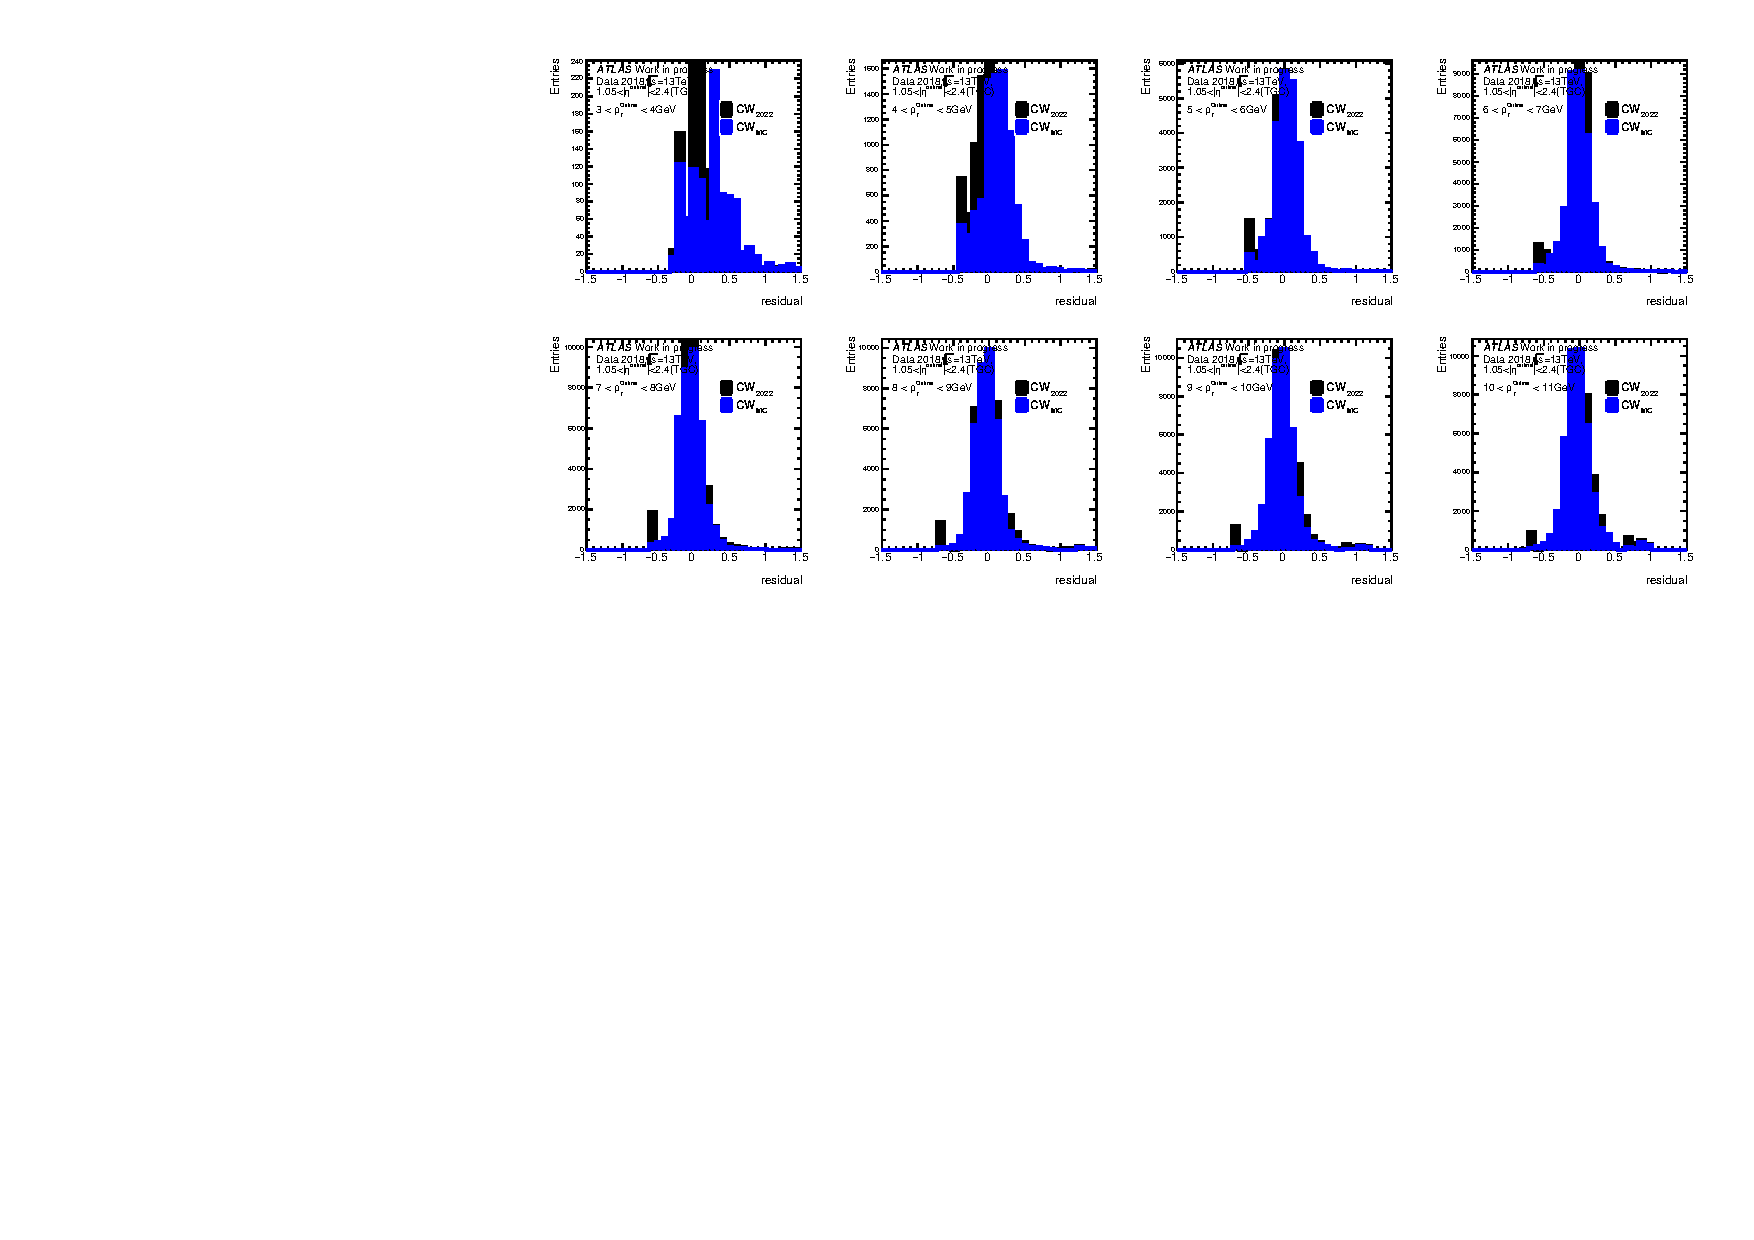
\includegraphics[clip, width=16cm]{fig/5/residual_MC_3_10.pdf}
  \caption{TGCにおける1GeV刻みのpT residual分布(3$\sim$10~GeV)。青が本研究の手法で作成した$\mathrm{CW_{Simu}}$を用いた結果、黒が2022年度Run-2で使用された$\mathrm{CW_{2022}}$を用いた結果である。}
  \label{residual_MC_3_10}
\end{figure}
\begin{figure}[htb]
  \centering
  %\rule{8cm}{6cm}
  \hspace*{-1cm}
  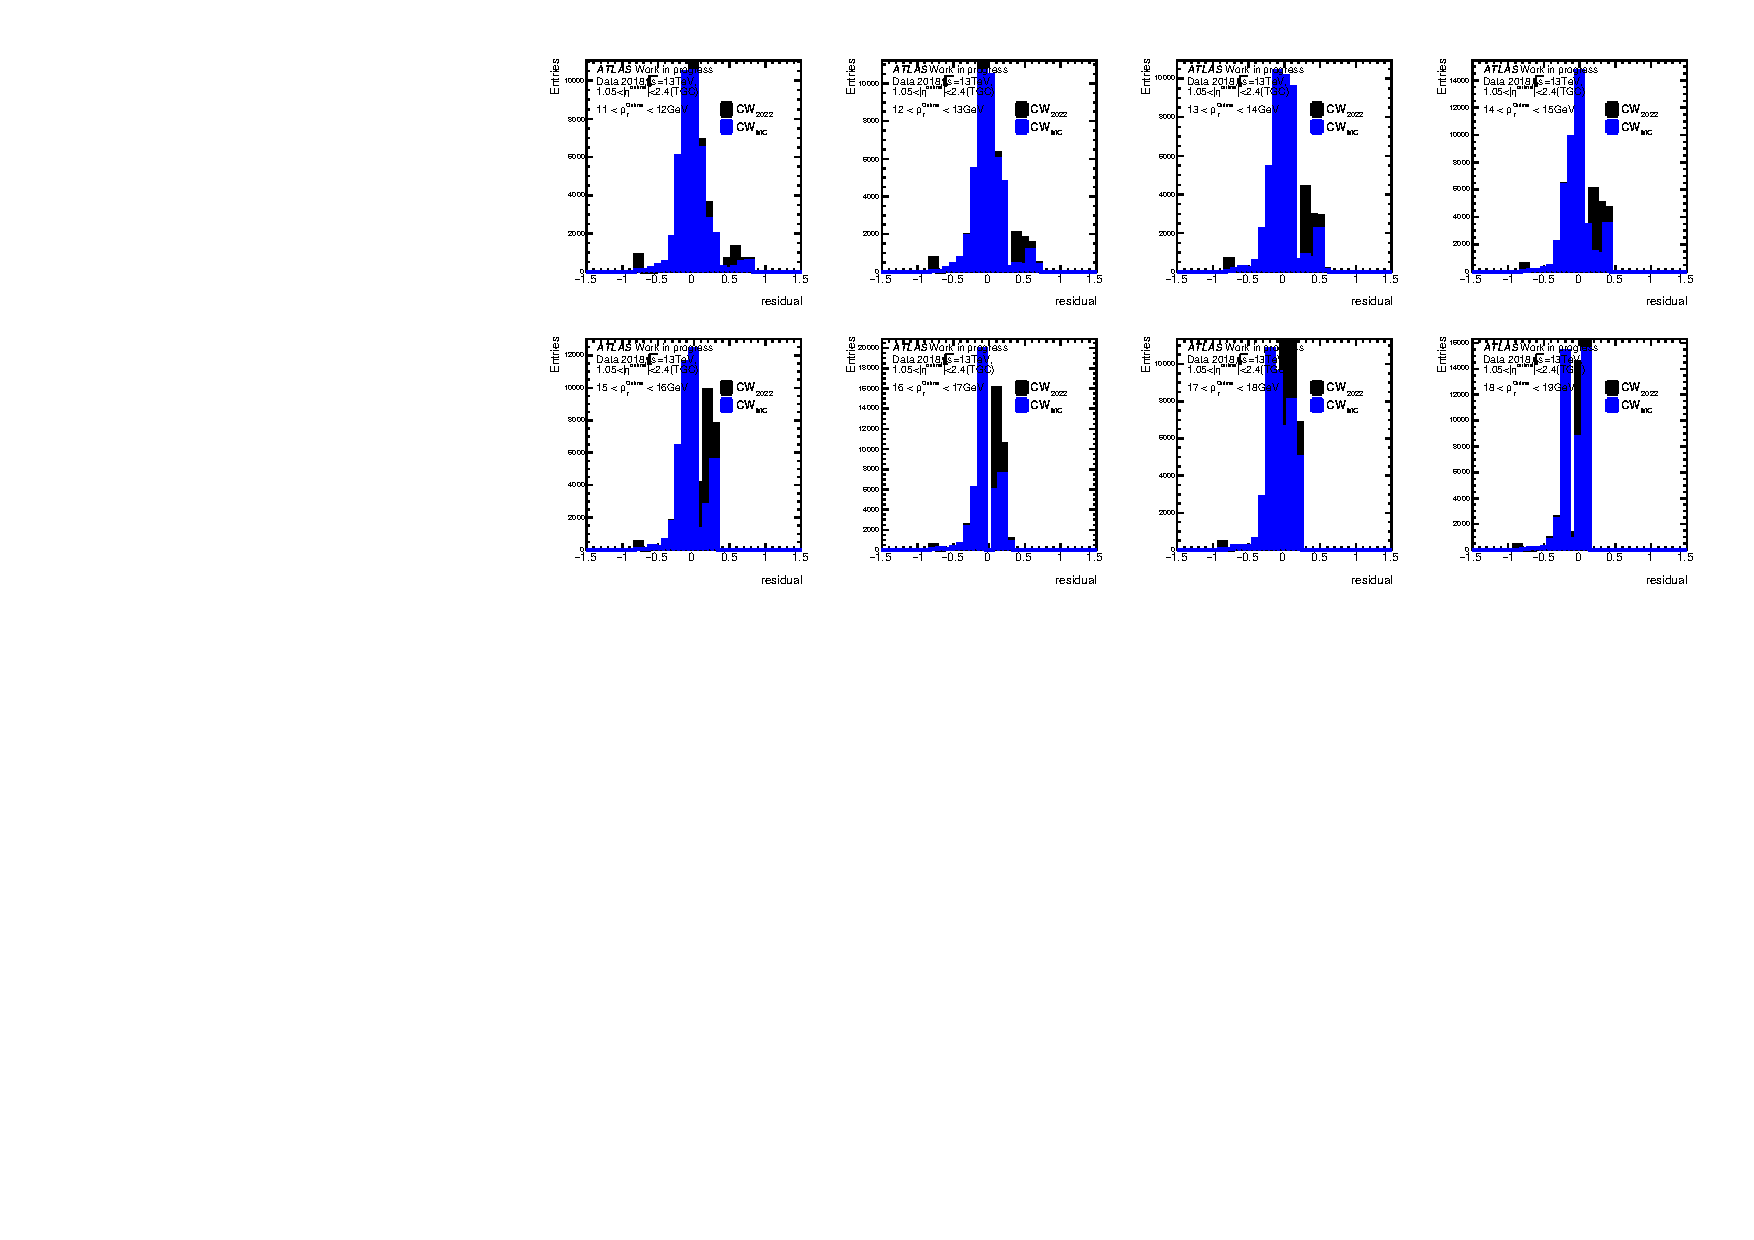
\includegraphics[clip, width=16cm]{fig/5/residual_MC_11_18.pdf}
  \caption{TGCにおける1GeV刻みのpT residual分布(11$\sim$18~GeV)。青が本研究の手法で作成した$\mathrm{CW_{Simu}}$を用いた結果、黒が2022年度Run-2で使用された$\mathrm{CW_{2022}}$を用いた結果である。}
  \label{residual_MC_11_18}
\end{figure}



次に、本研究の手法で作成した$\mathrm{CW_{Data}}$と2022年度Run-2で使用された$\mathrm{CW_{2022}}$の比較を行う。
評価には2022年Run-2のデータを用いる。
図~\ref{residual_Data_3_10}と図~\ref{residual_Data_11_18}に1~GeVごとの$p_{\rm{T}}^{offline}$に対する$p_{\rm{T}}$ residual分布を示す。
本研究の手法で作成した$\mathrm{CW_{Data}}$は、2022年度Run-2で使用された$\mathrm{CW_{2022}}$と同様の分布を示している。
\begin{figure}[htb]
  \centering
  %\rule{8cm}{6cm}
  \hspace*{-1cm}
  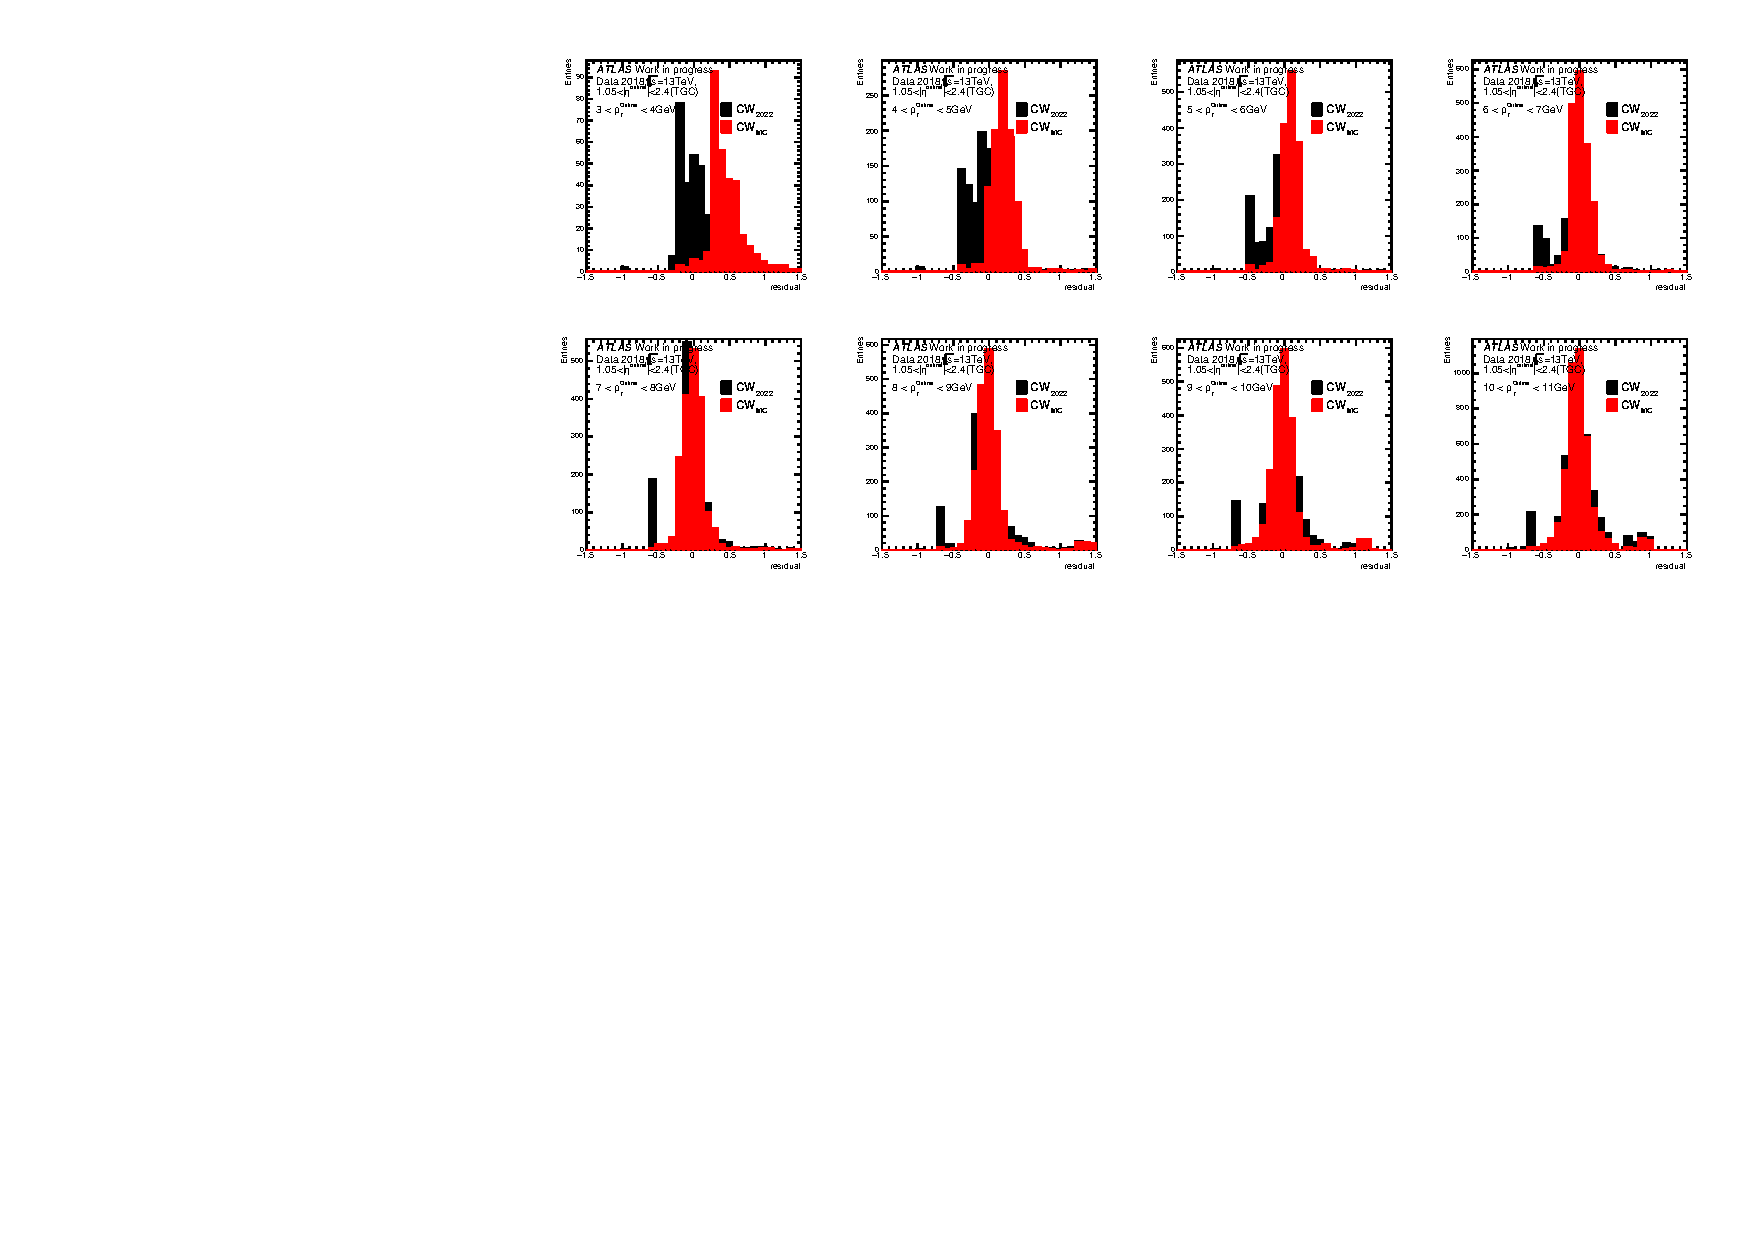
\includegraphics[clip, width=16cm]{fig/5/residual_Data_3_10.pdf}
  \caption{TGCにおける1GeV刻みのpT residual分布(3$\sim$10~GeV)。赤が本研究の手法で作成した$\mathrm{CW_{Data}}$を用いた結果、黒が2022年度Run-2で使用された$\mathrm{CW_{2022}}$を用いた結果である。}
  \label{residual_Data_3_10}
\end{figure}
\begin{figure}[htb]
  \centering
  %\rule{8cm}{6cm}
  \hspace*{-1cm}
  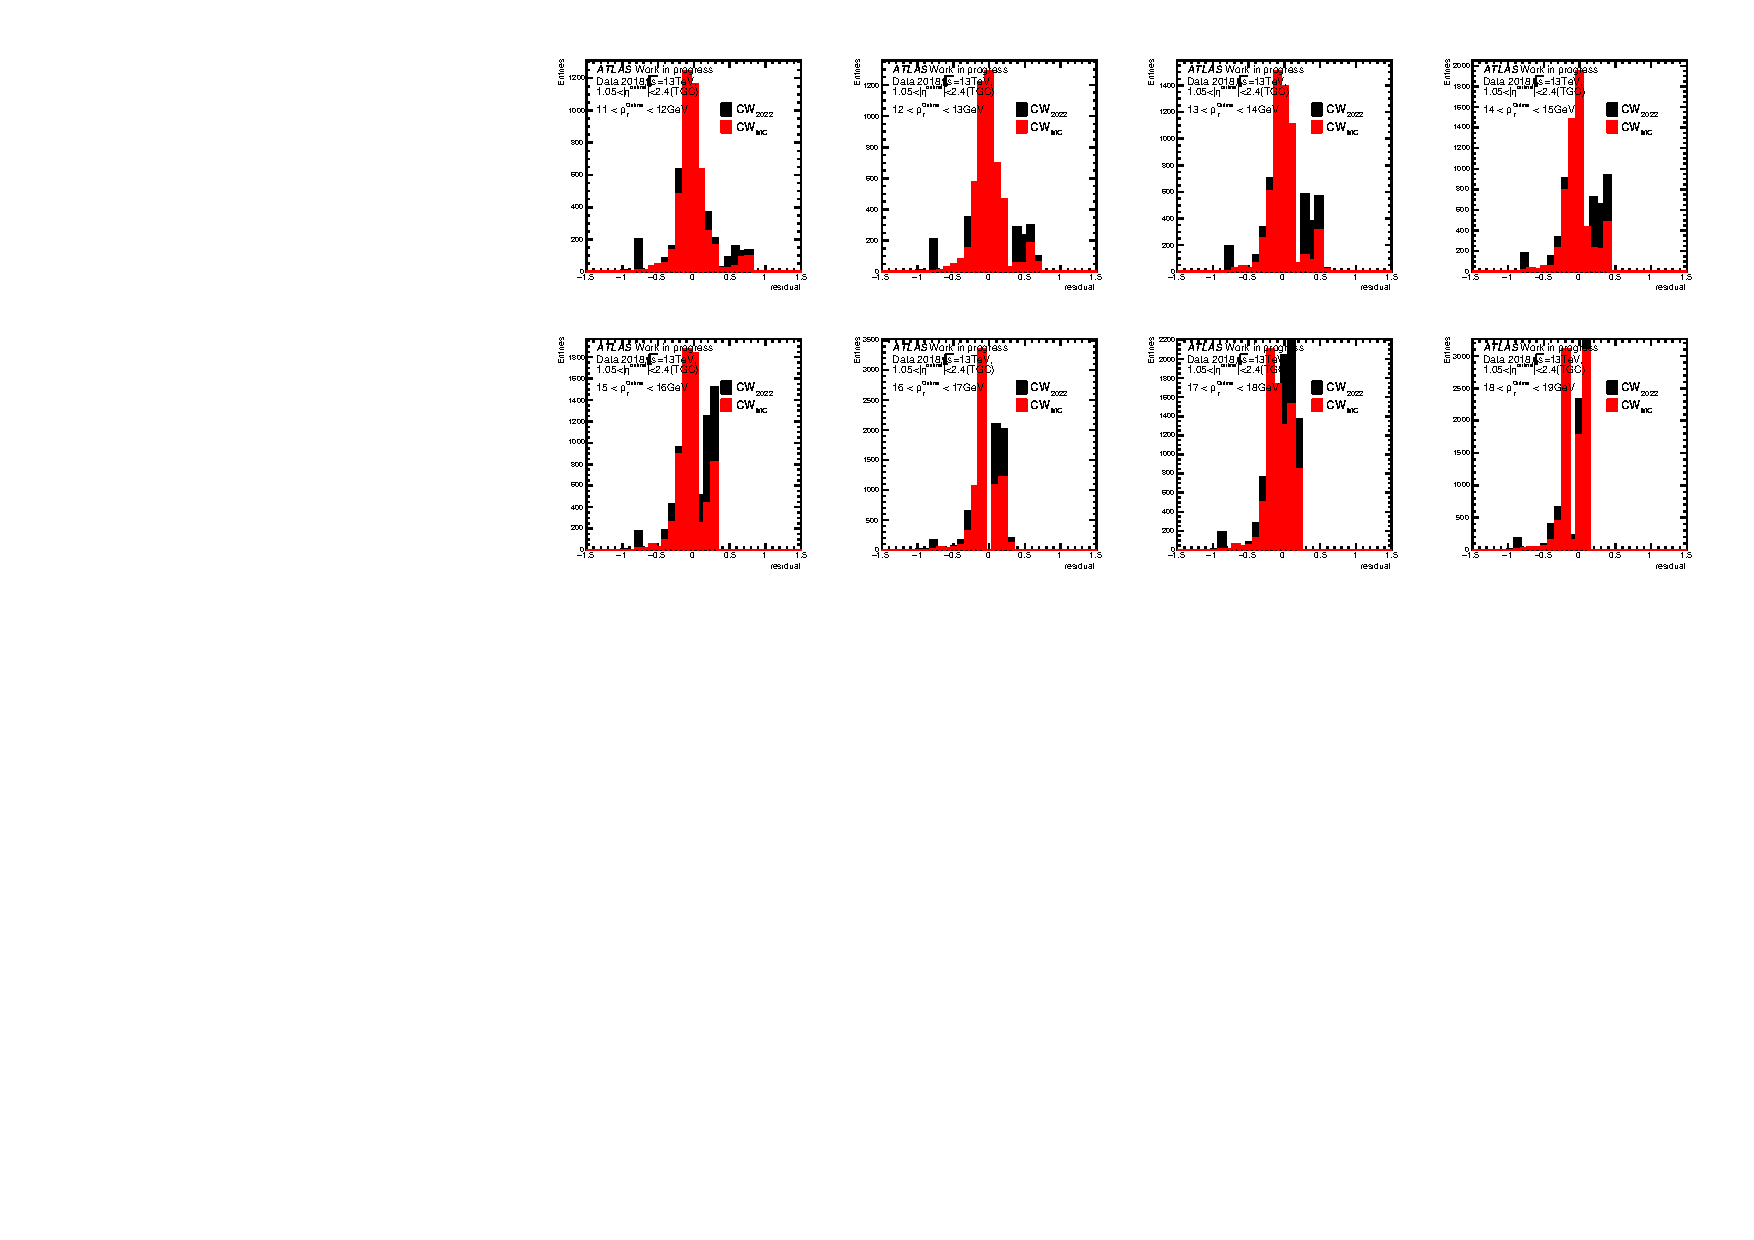
\includegraphics[clip, width=16cm]{fig/5/residual_Data_11_18.pdf}
  \caption{TGCにおける1GeV刻みのpT residual分布(11$\sim$18~GeV)。赤が本研究の手法で作成した$\mathrm{CW_{Data}}$を用いた結果、黒が2022年度Run-2で使用された$\mathrm{CW_{2022}}$を用いた結果である。}
  \label{residual_Data_11_18}
\end{figure}


\subsection{機械学習によるCWの最適化の評価}
実際のデータを機械学習に用いることで期待されるCWの最適化の効果について評価を行う。

本研究で開発した手法では、実際のデータをトレーニング用いることで自動で最適化を行うことで$\mathrm{CW_{Data}}$と$\mathrm{CW_{Simu}}$を作成した。そのため、最適化を行っていない$\mathrm{CW_{2022}}$よりもトリガー性能が向上することが期待される。

まず、検出器アライメントに対応してCWをズラすことができているかを確認する。
8回転対象の磁場構造において、同じ磁場構造となる場所に位置するRoIのCWの、$p_{\rm{T}}$閾値が14~GeVとなる領域についての$\mathrm{CW_{Data}}$と$\mathrm{CW_{2022}}$の比較を図~\ref{fig:CWv05v07}に示す。
図~\ref{fig:CWv05v07}に示す8個のCWは、シミュレーション上では磁場構造が同じになるため、黒枠で表される$\mathrm{CW_{2022}}$はすべて同じ形である。しかし、\ref{ズレ}節で述べたように、実際の検出器のズレによって場所によって磁場構造が異なるため、本手法で作成した$\mathrm{CW_{Data}}$ではCWに数マス分のズレが生じている。
\begin{figure}[tb]
  \centering
  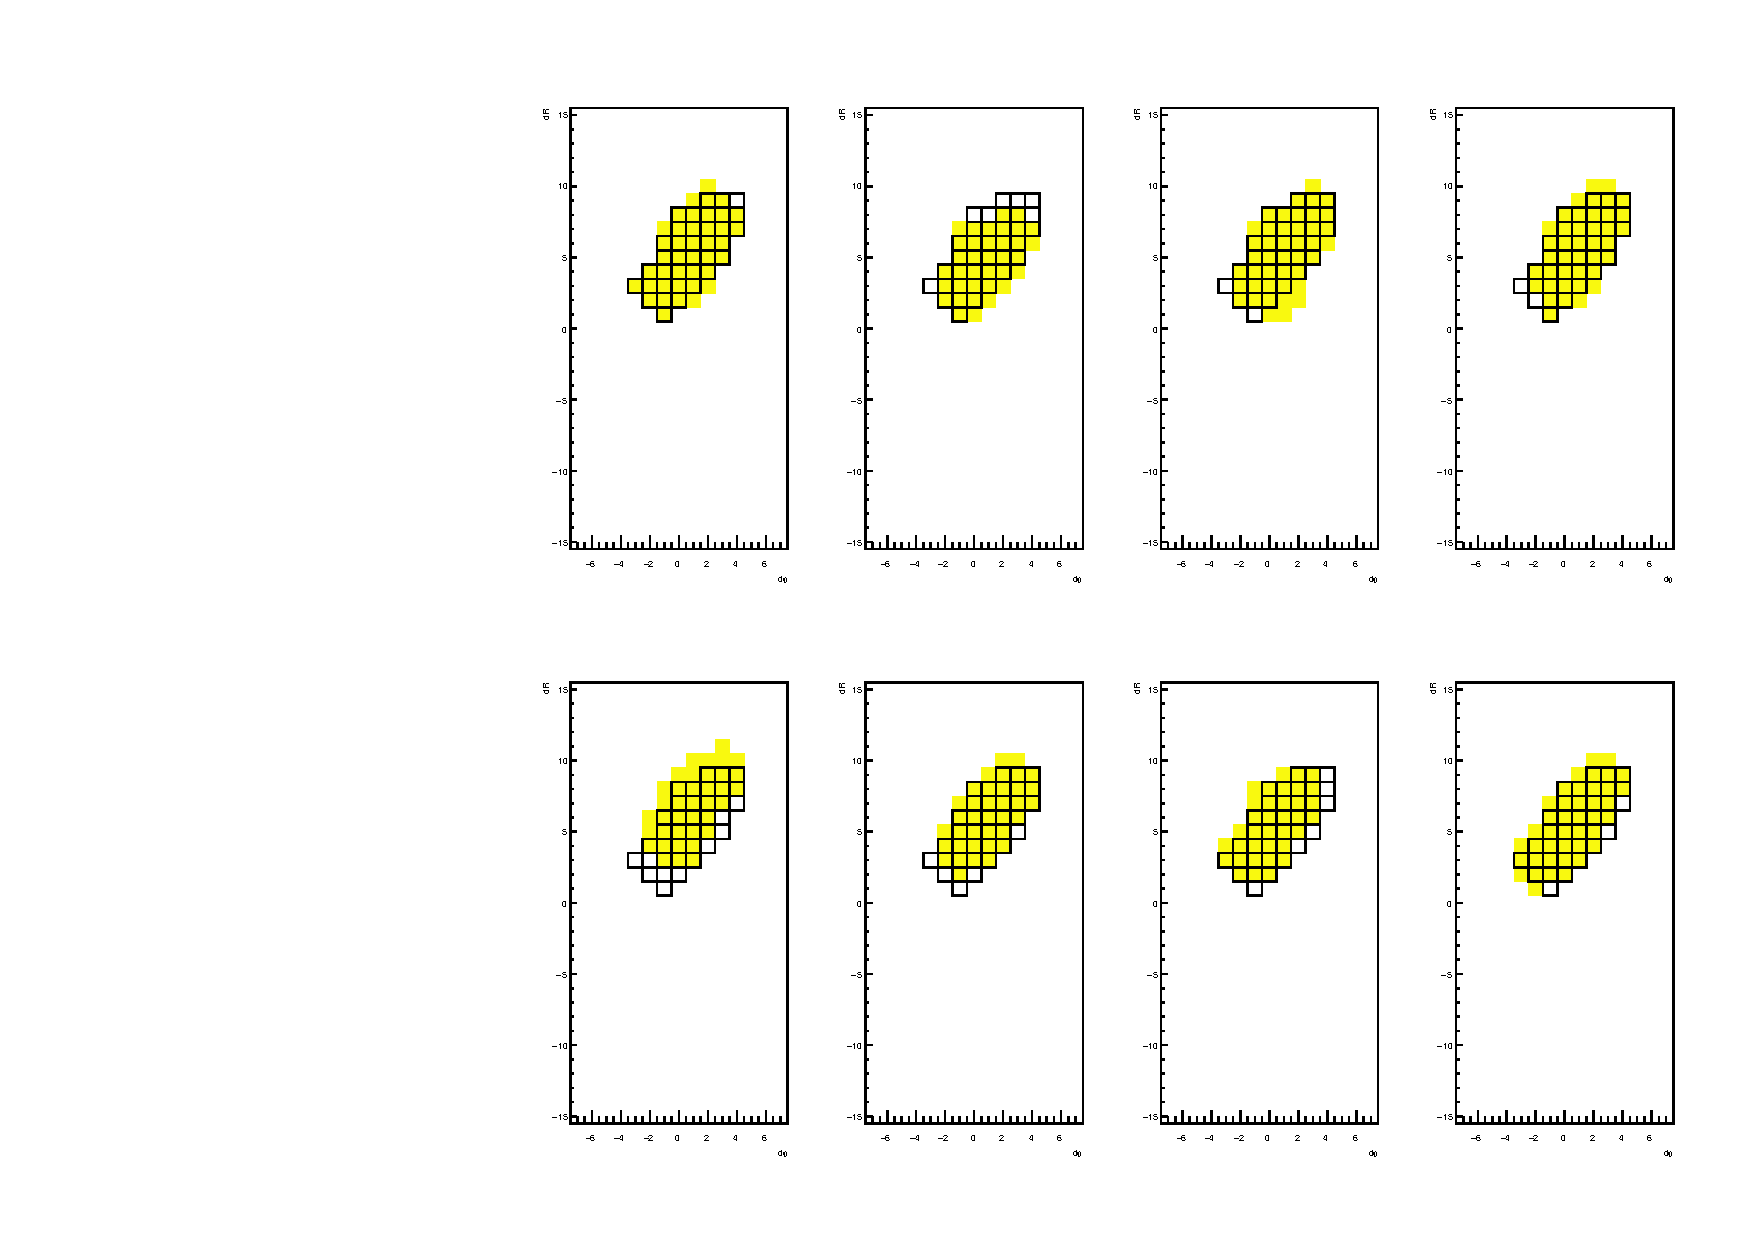
\includegraphics[clip, width=13cm]{fig/5/ALL_Aside_Endcap_phiSector_Octant1_roi58.pdf}
  \caption{$p_{\rm{T}}$閾値が14~GeVとなる領域の比較。黄色の領域が本手法で作成した$\mathrm{CW_{Data}}$、黒枠の領域が$\mathrm{CW_{2022}}$である。}
  \label{fig:CWv05v07}
\end{figure}

次に、2018年Run-2データを評価に用いた際の$\mathrm{CW_{Data}}$と$\mathrm{CW_{Simu}}$の比較を行う。図~\ref{fig:v06v07}に$p_{\rm{T}}$閾値14~GeVにおけるTurn-on curveを比較したプロットを示す。実際のデータに対して、$\mathrm{CW_{Data}}$を用いたトリガーの方がトリガー効率が良くなっているのが見て取れる。
\begin{figure}[tb]
  \centering
  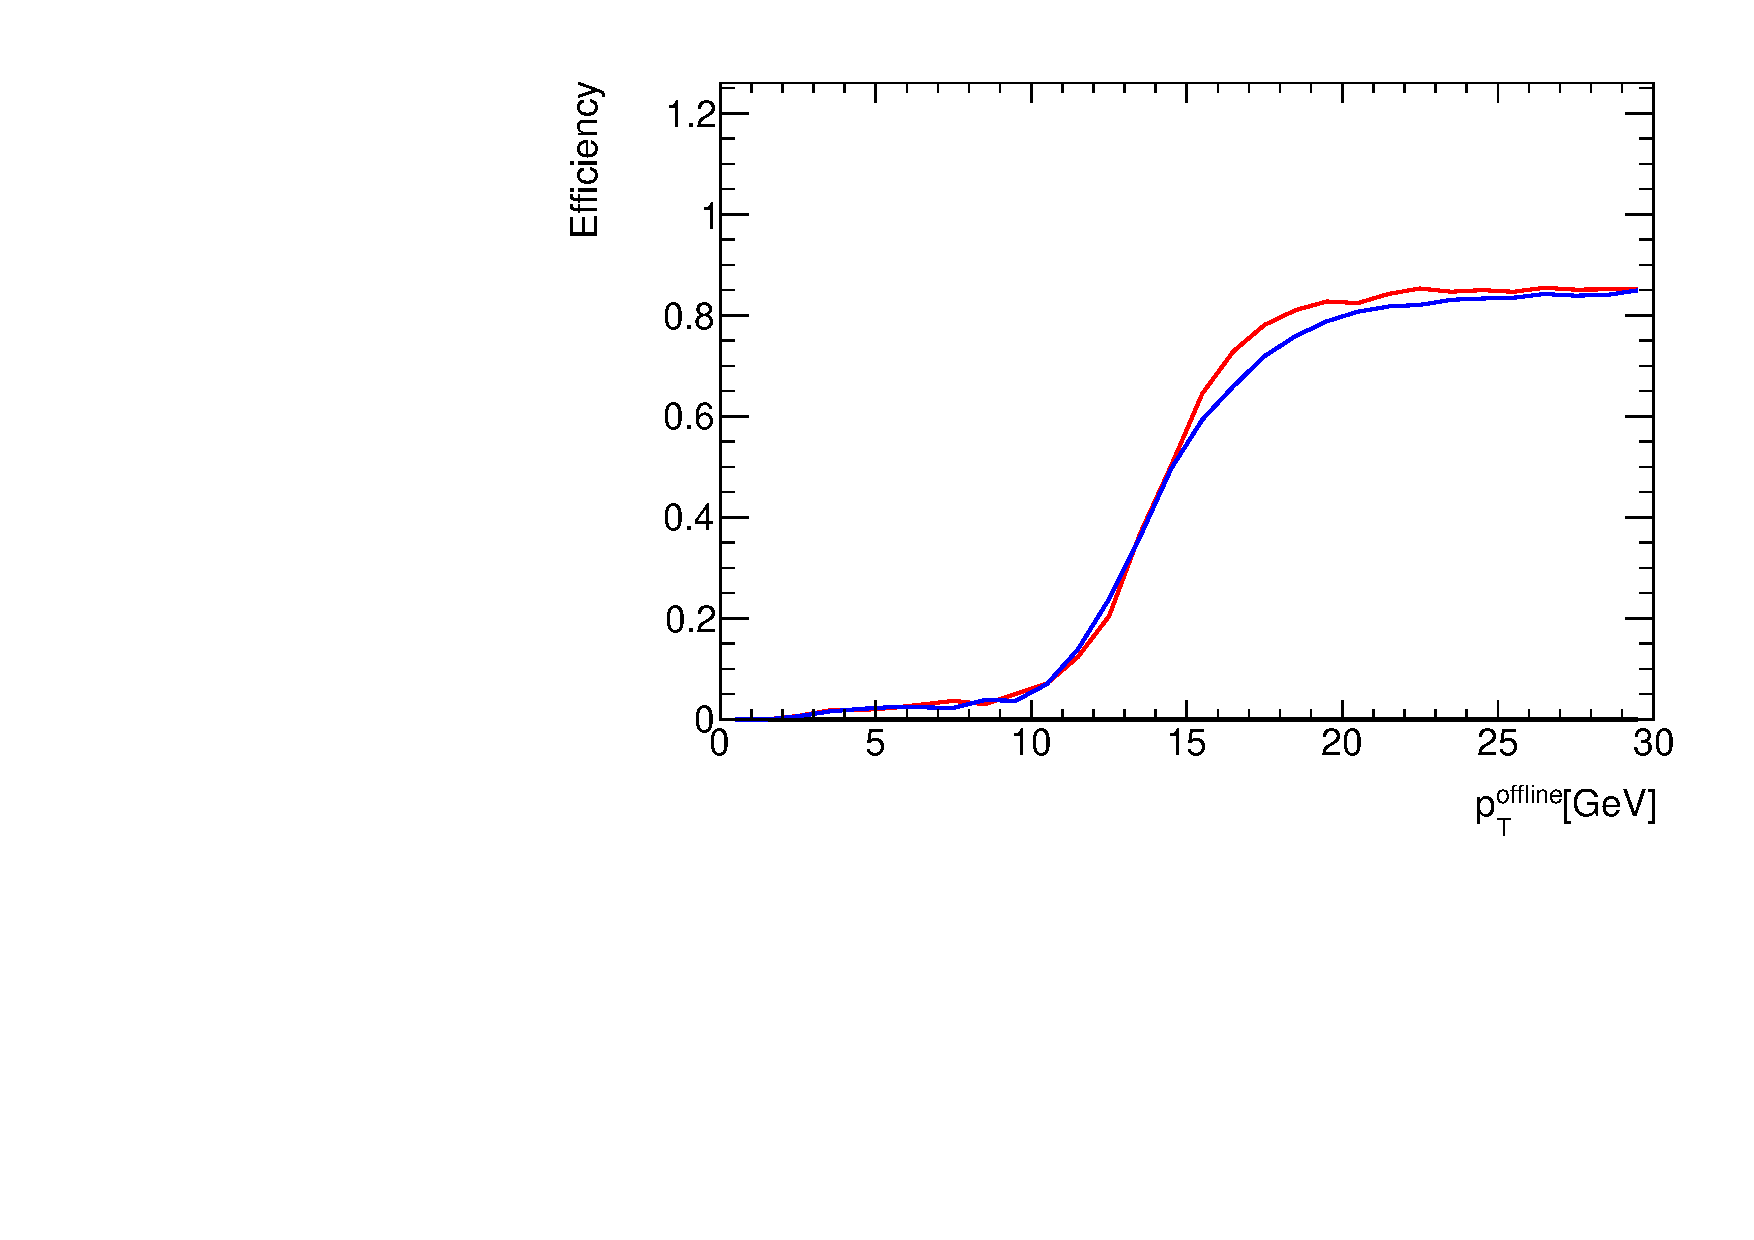
\includegraphics[clip, width=11cm]{fig/4/v06vsv07_MU14.pdf}
  \caption{$\mathrm{CW_{Data}}$と$\mathrm{CW_{Simu}}$のTurn-on curve。$p_{\rm{T}}$閾値14~GeVのトリガー効率の比較を行い、評価には2018年Run-2データを使用した。}
  \label{fig:v06v07}
\end{figure}

%\begin{figure}[h]
%  \centering
%  %\rule{8cm}{6cm}
%  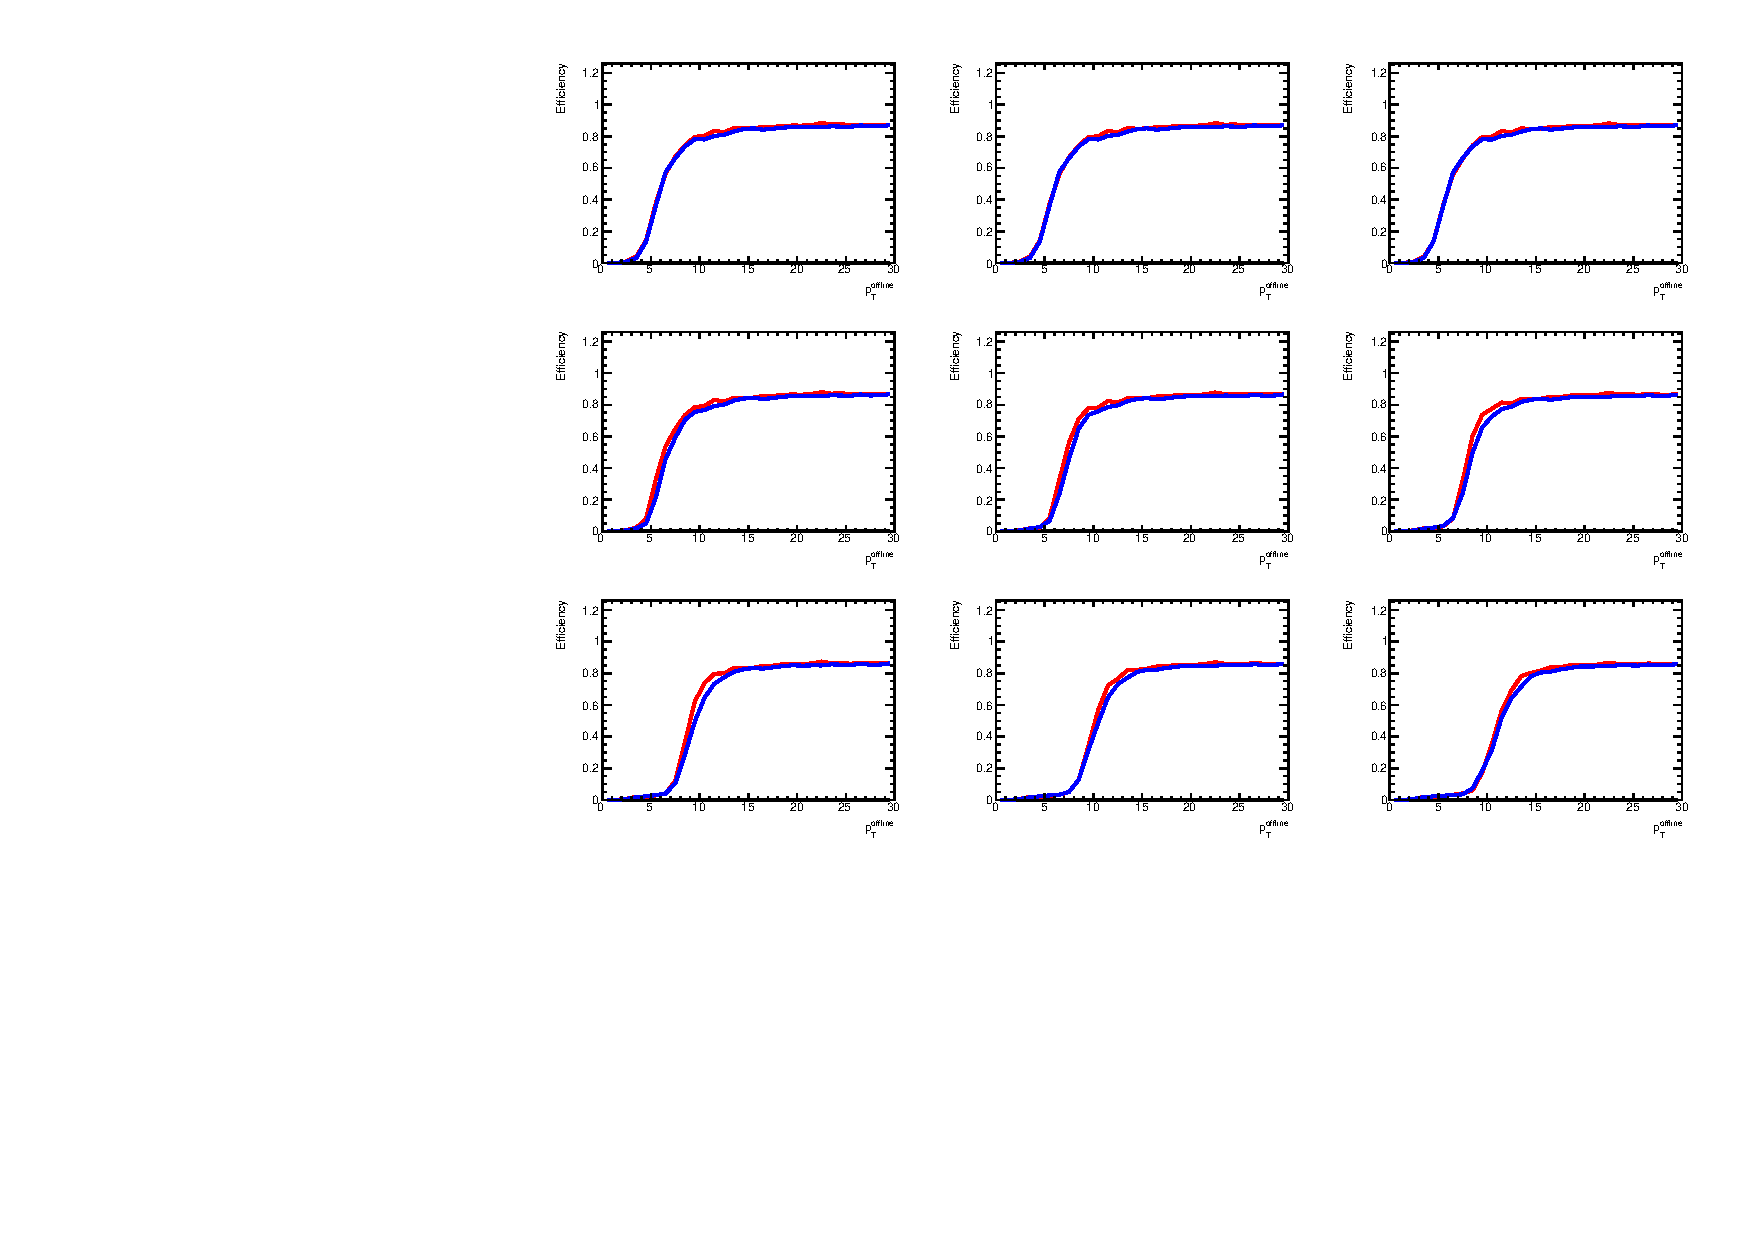
\includegraphics[clip, width=11cm]{fig/5/v06v07_1_15.pdf}
%  \caption{$\mathrm{CW_{Data}}$と$\mathrm{CW_{Simu}}$のTurn-on curveの比較。$p_{\rm{T}}$閾値3~GeVから14~GeVまでのトリガー効率の比較を行い、評価には2018年Run-2データを使用した。}
%  \label{fig:v06v07_1_9}
%\end{figure}

%\begin{figure}[h]
%  \centering
%  %\rule{8cm}{6cm}
%  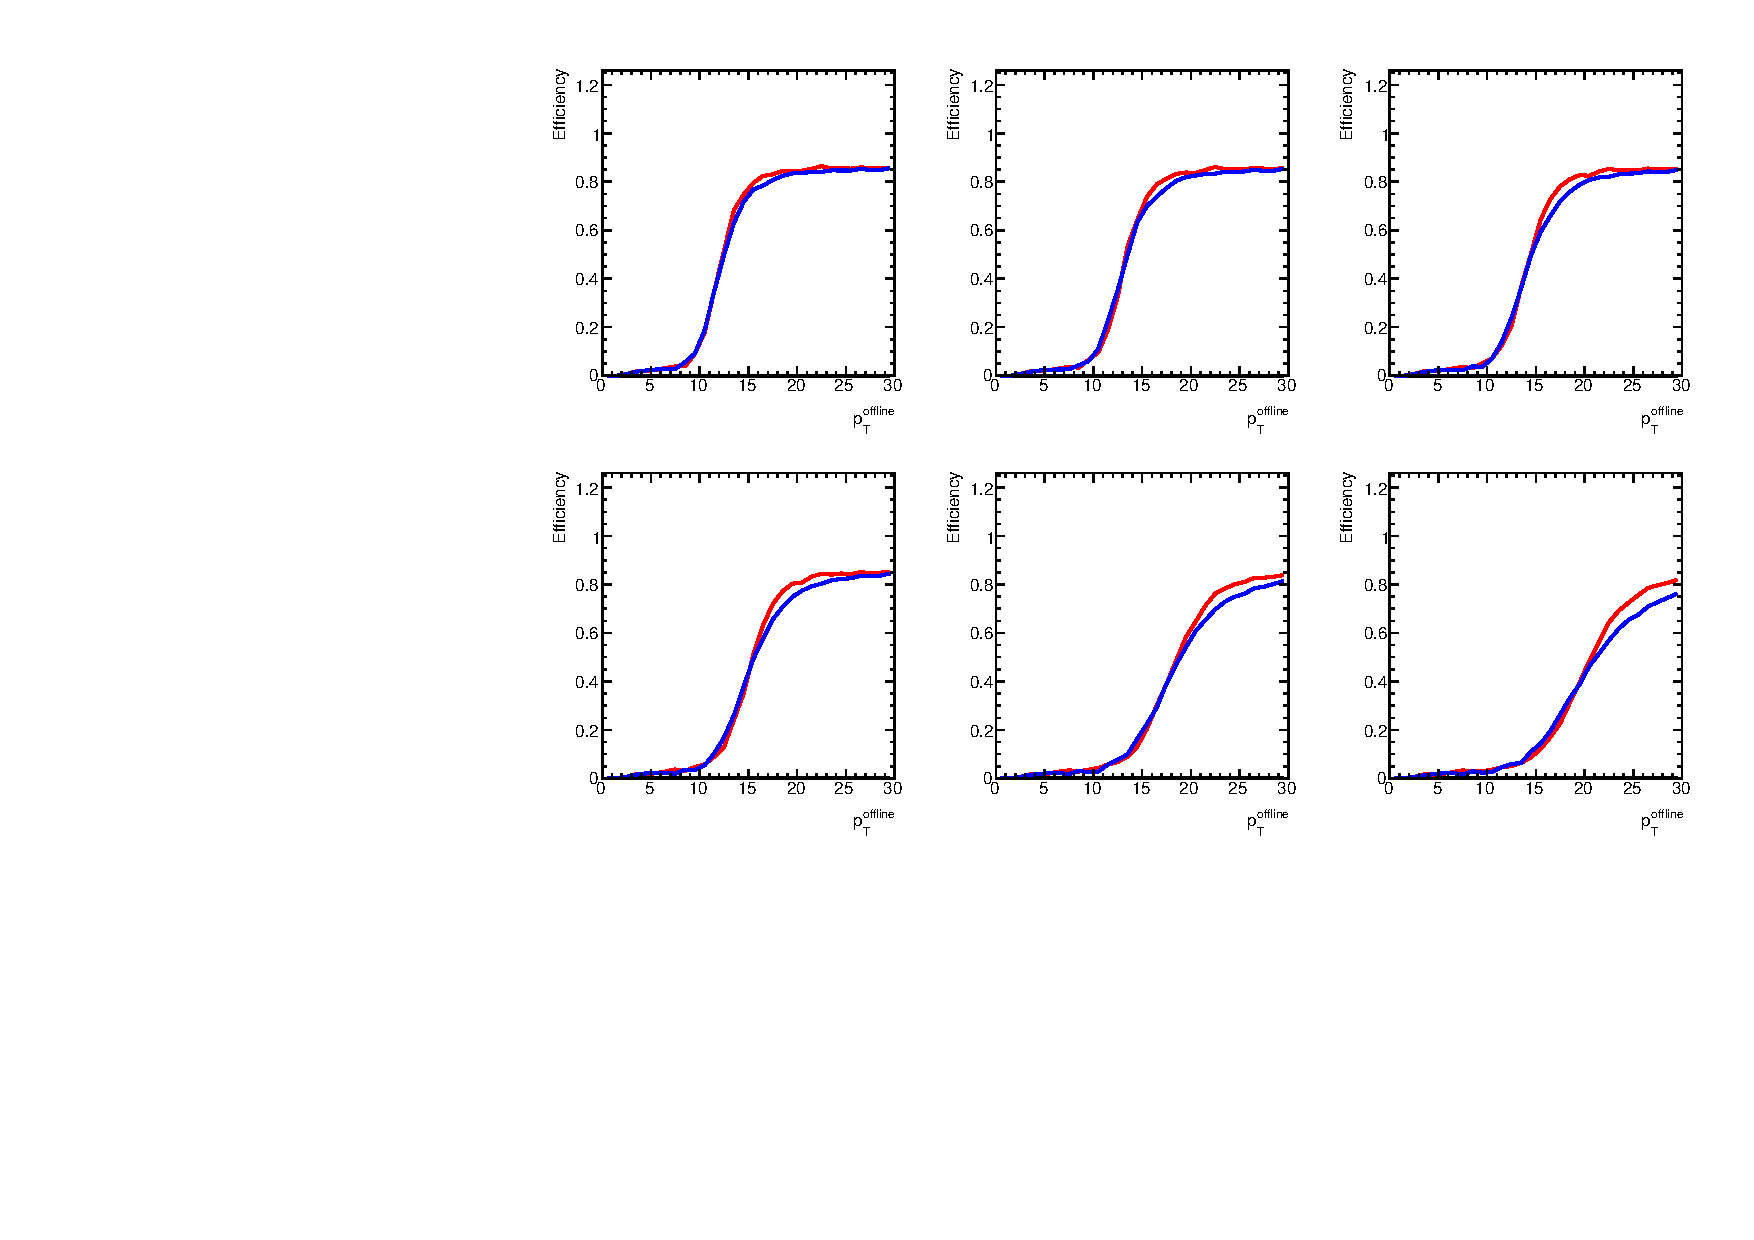
\includegraphics[clip, width=10cm]{fig/5/v06v07_10_15.pdf}
%  \caption{$\mathrm{CW_{Data}}$と$\mathrm{CW_{Simu}}$のTurn-on curveの比較。$p_{\rm{T}}$閾値15~GeVから20~GeVまでのトリガー効率の比較を行い、評価には2018年Run-2データを使用した。}
%  \label{fig:v06v07_12_20}
%\end{figure}

%\subsubsection{ミューオン電荷に対するトリガー性能の評価}
さらに、TGCチェンバーごとにミューオンの電荷別のトリガー効率の評価を行った。
あるチェンバーにおける$\mathrm{CW_{Data}}$と$\mathrm{CW_{2022}}$電荷別のトリガー効率を図~\ref{Eff_Chage}に示す。
図~\ref{fig:v05_charge}に示すように、$\mathrm{CW_{2022}}$は検出器のズレに対する補正を行っていないために、ミューオンの電荷別に計算したトリガー効率に大きな差が出る。
一方、図~\ref{fig:v06_charge}に示すように、本研究の手法で作成した$\mathrm{CW_{Data}}$はCWが最適化されたことにより、電荷別に計算したトリガー効率がほとんど一致していることが見て取れる。
\begin{figure}
    %\centering
    \begin{tabular}{cc}
    \begin{minipage}[b]{0.45\hsize}
        %\centering
        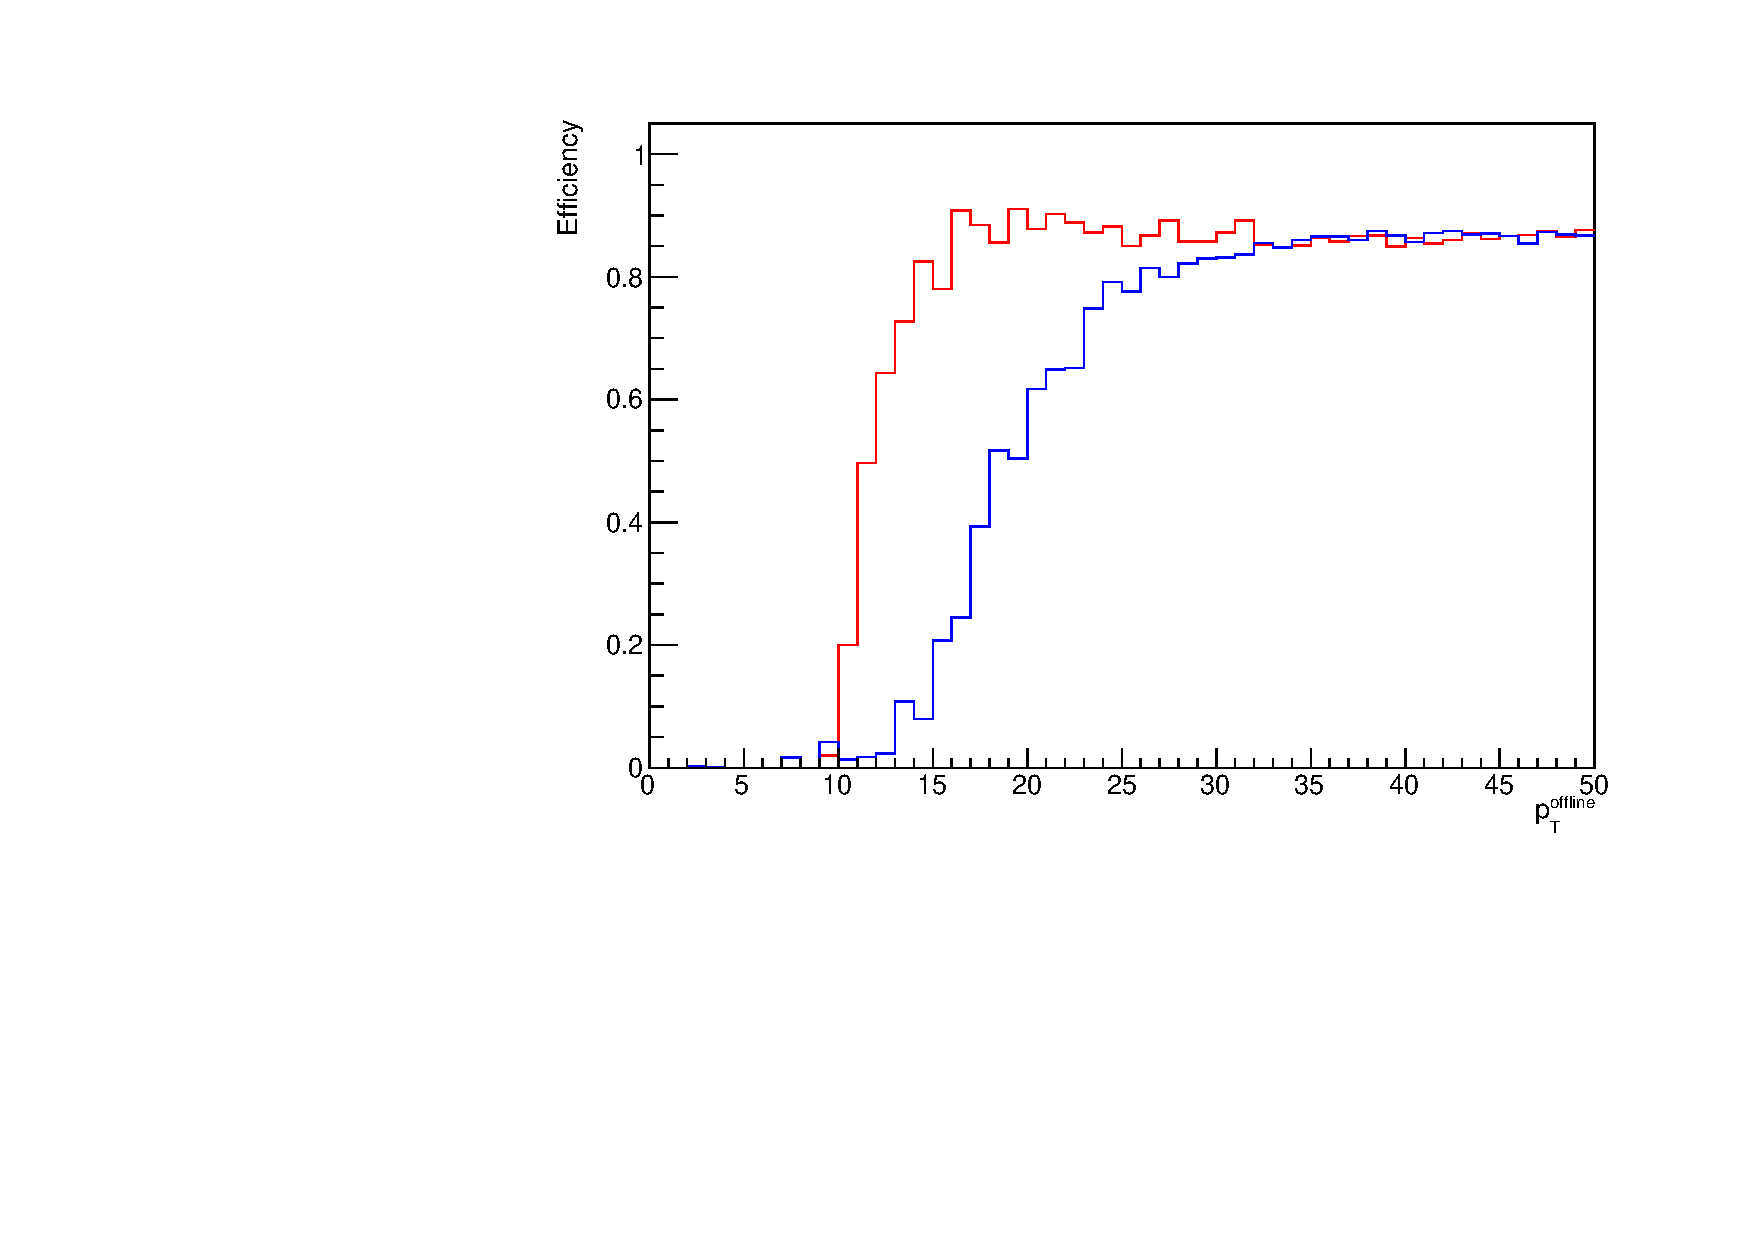
\includegraphics[clip, width=7cm]{fig/5/Eff_PNcharge_v05_phi0eta10.pdf}
        %\vspace{5pt}
        \subcaption{}
        \label{fig:v05_charge}
    \end{minipage}&
    %\hfill
    \begin{minipage}[b]{0.45\hsize}
        %\centering
        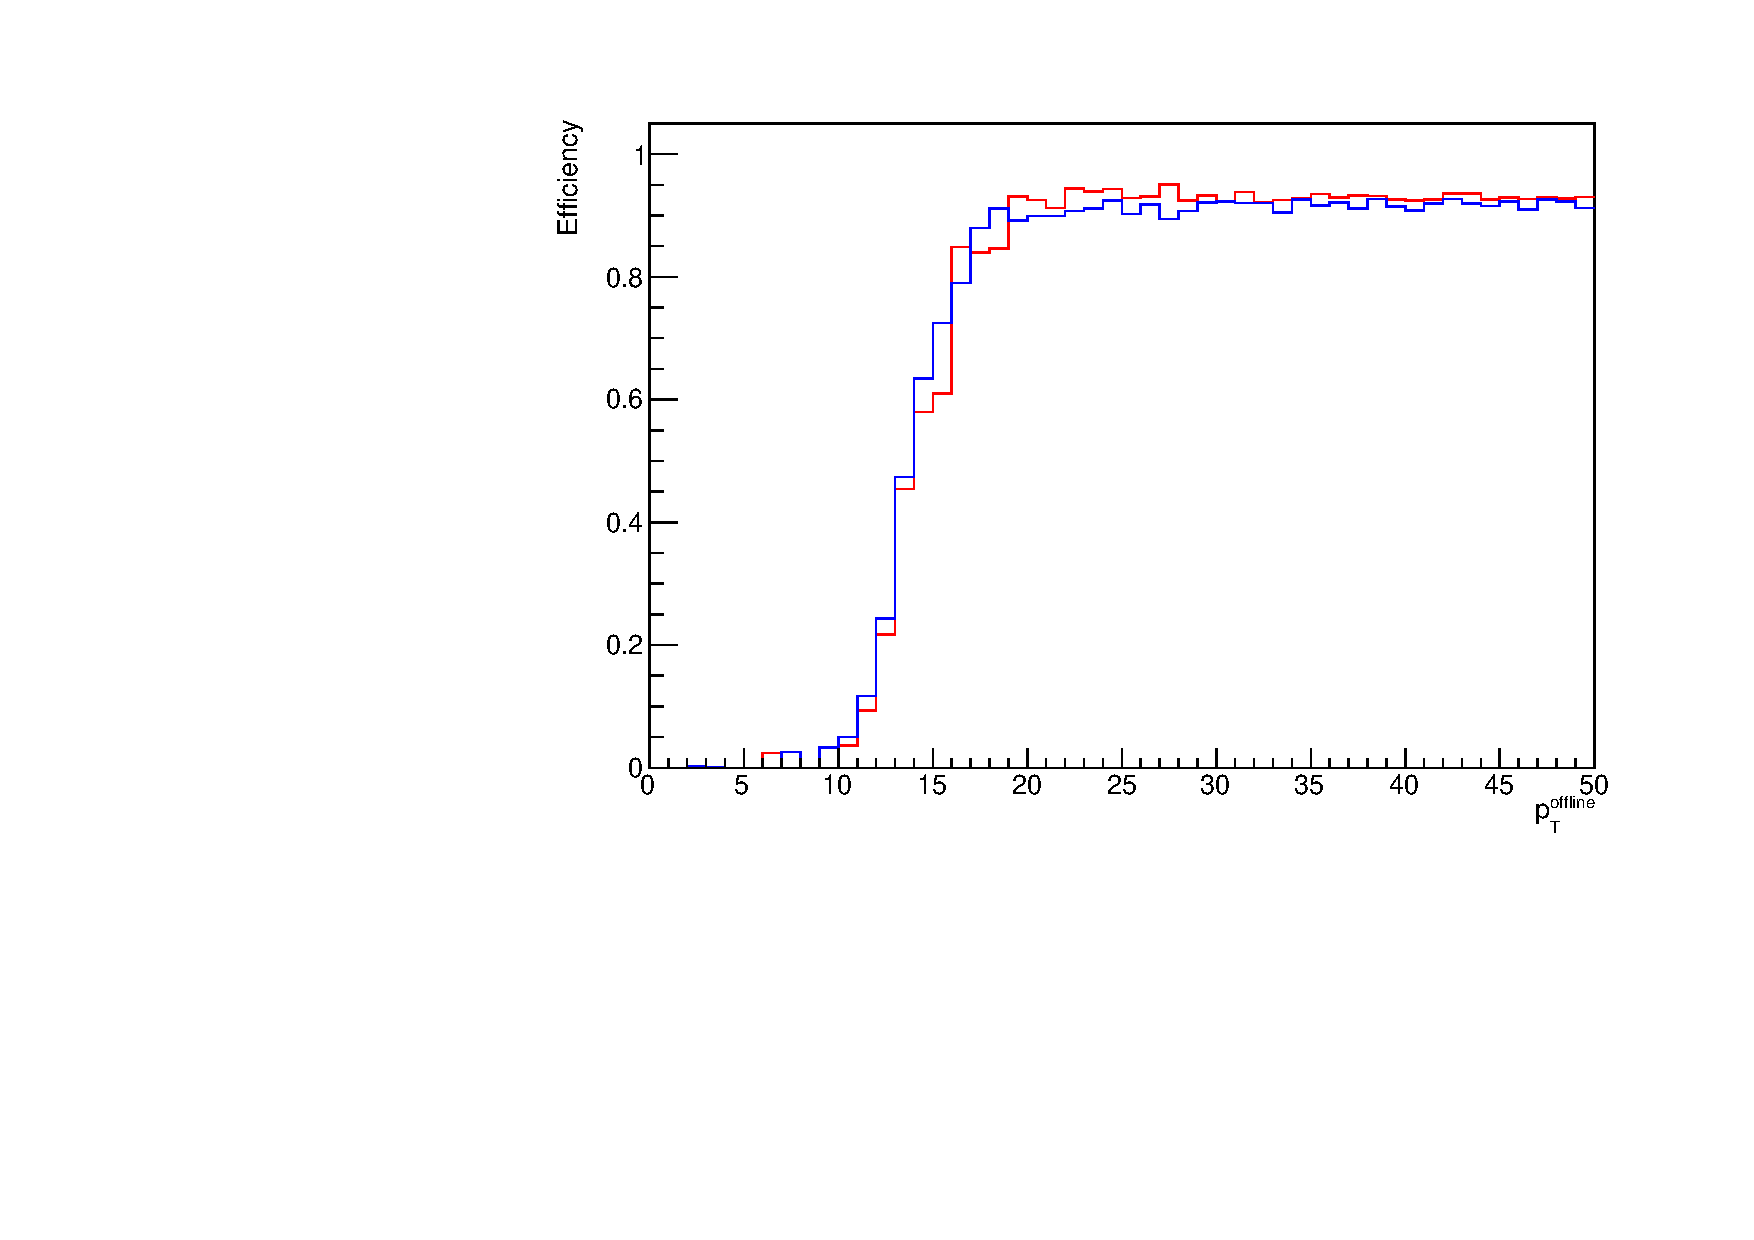
\includegraphics[clip, width=7cm]{fig/5/Eff_PNcharge_MLP_phi0eta10.pdf}
        %\vspace{5pt}
        \subcaption{}
        \label{fig:v06_charge}
    \end{minipage}
    \end{tabular}
    \caption{あるチェンバーにおける電荷別に計算した$p_{\rm{T}}$閾値14~GeVのTurn-on curveの比較。赤が正電荷、青が負電荷。(a):$\mathrm{CW_{2022}}$(b):$\mathrm{CW_{Data}}$}
    \label{Eff_Chage}
\end{figure}
本研究の手法では、実際のデータを機械学習のトレーニングに用いたことで、TGC 検出器の位置による磁場構造の違いや検出器のズレを自動で補正することができ、CWが最適化されたことを示している。



%\newpage
%\newpage

%\subsubsection{TGCのチェンバーごとの領域でのトリガー性能}
%さらに、TGC チェンバーごとにトリガー効率を算出し、Turn-on curveに対してフィッティングを行う。

%\begin{figure}[tb]
%  \centering
%  \rule{8cm}{6cm}
  %\includegraphics[clip, width=14cm]{}
%  \caption{チェンバーごとのEfficiency (1-48)}
%  \label{fig:fit_def}
%\end{figure}





\subsection{トリガーレートの評価}
次に、本手法で作成したCWを使用したときのトリガーレートの評価を行う。トリガーレートとは、実験データにおけるトリガーが発行された事象数である。
2018年のRun-2データを用いてトリガーレートを計算する。
Run-2データにはHLTでのプリスケールによるバイアスが存在するため、バイアスのない状態でトリガーレートを計算するために、「HLT$\_$noalg$\_$L1MU4」を要求する。このトリガーはL1 TriggerにおいてpT閾値が4GeV以上を要求するが、HLTによる事象選別のない(Passthrough)トリガーチェインである。
その後、HLT$\_$noalg$\_$L1MU4が鳴ったイベントの中でL1$\_$MU$x$が鳴ったイベントがいくら存在するかを調べ、ルミノシティが***の時のL1$\_$MU4のトリガーレート(***kHz)をかけることでMUxのトリガーレートを見積もる。式~\eqref{equ:トリガーレート}にトリガーレートの計算式を示す。
\begin{equation}
    \rm{MU}xのレート[\rm{kHz}] = \frac{\rm{MU}xが鳴ったイベント数}{HLT\_noalg\_L1MU4が鳴った全イベント数}\times L1\_MU4のレート[kHz]
    \label{equ:トリガーレート}
\end{equation}
図~\ref{fig:Ratev05v06}に2016年で取得されたデータを用いて算出したトリガーレートを示す。

\begin{figure}[tb]
  \centering
  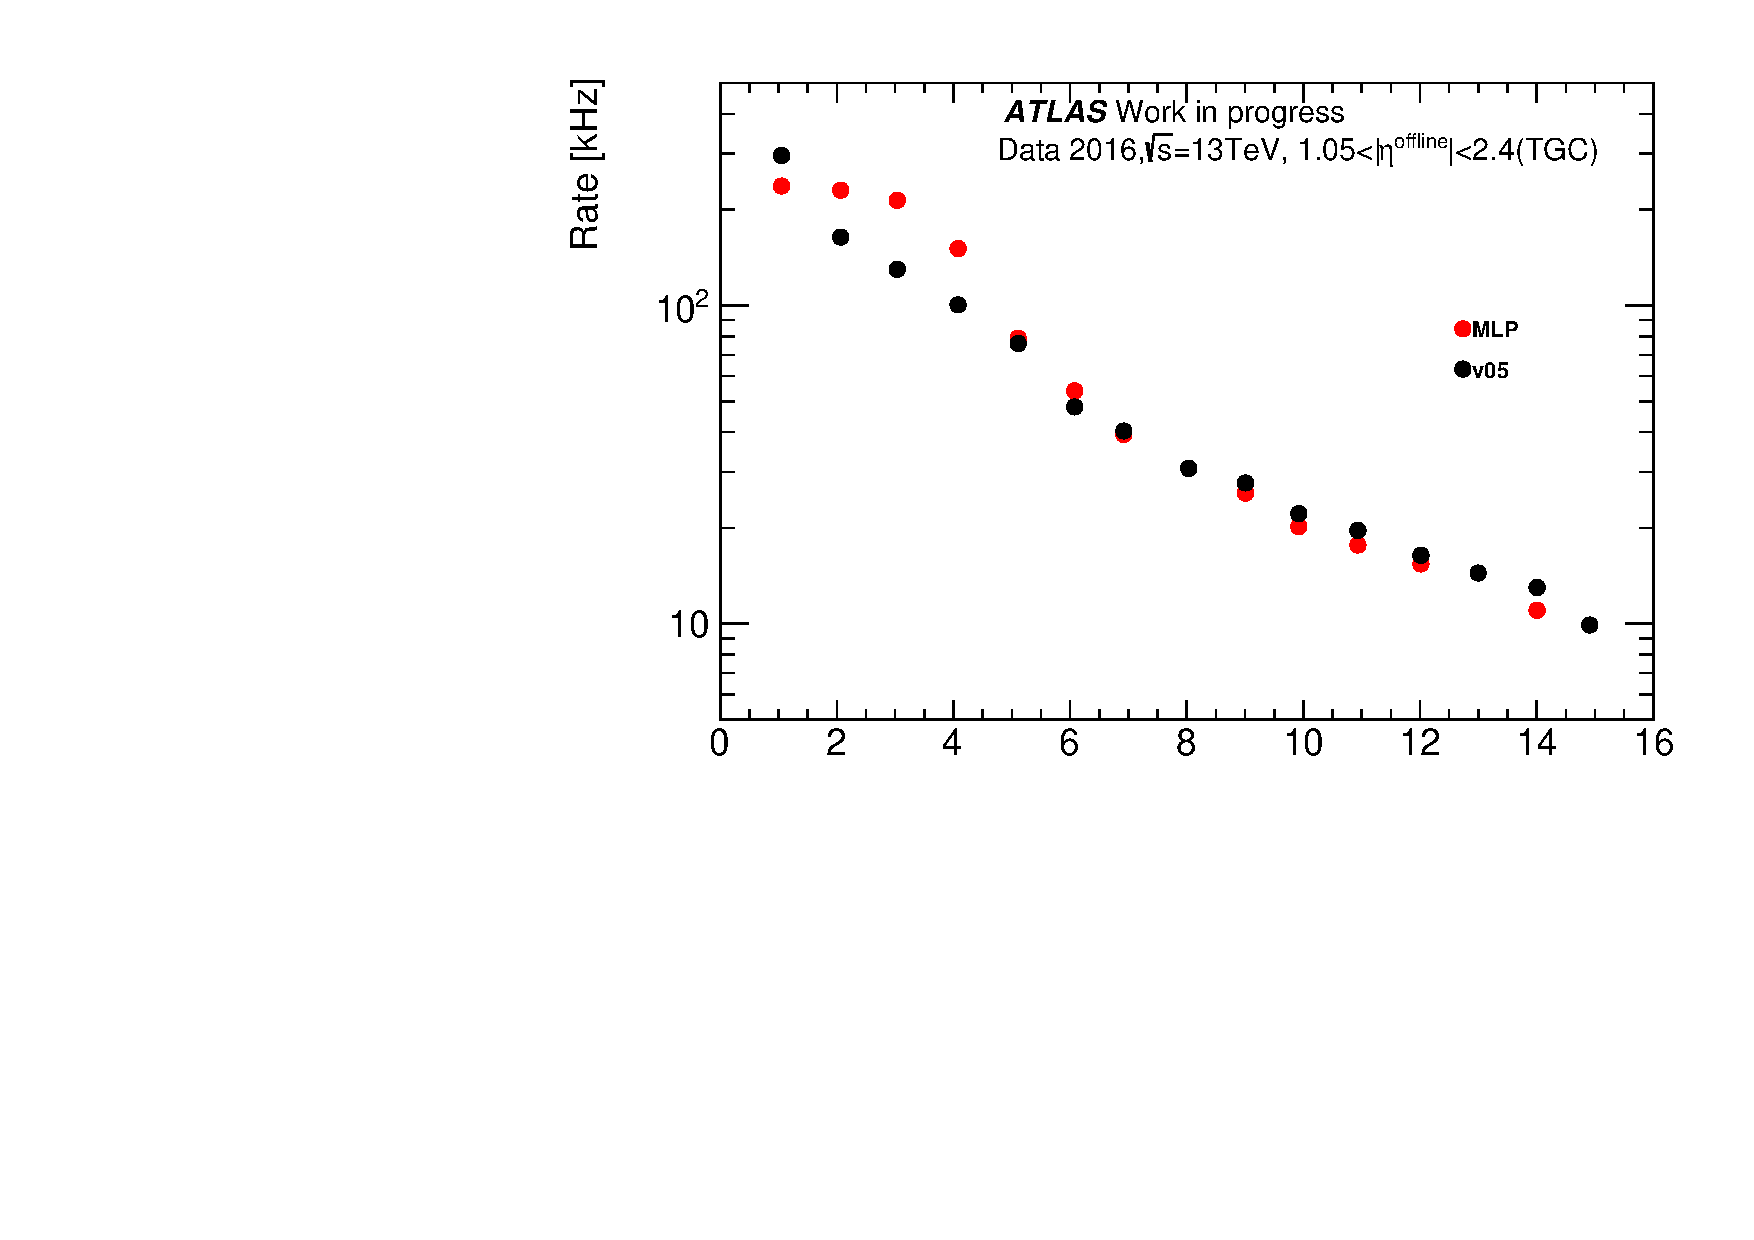
\includegraphics[clip, width=11cm]{fig/5/15rate.pdf}
  \caption{TGCにおけるシングルミューオンのトリガーレート。}
  \label{fig:Ratev05v06}
\end{figure}

$p_{\rm{T}}$閾値7~GeV以上のトリガーにおいて、$\mathrm{CW_{Data}}$のトリガーレートの値は$\mathrm{CW_{2022}}$と同等であることが見て取れる。
しかし、$p_{\rm{T}}$閾値4~GeV、5~GeV、6~GeVのトリガーに関してはトリガーレートの大幅な増加が見られる。
